\documentclass[12pt]{article}
\usepackage{amsmath,amssymb,amsthm}
\usepackage{graphicx,psfrag,epsf}
\usepackage{enumerate}
\usepackage[square,numbers]{natbib}
\usepackage{bm}
\usepackage{algorithm}
\usepackage{algpseudocode}

\newcommand{\blind}{0}
\newtheorem{theorem}{Theorem}
\newtheorem{lemma}{Lemma}

\addtolength{\oddsidemargin}{-.75in}%
\addtolength{\evensidemargin}{-.75in}%
\addtolength{\textwidth}{1.5in}%
\addtolength{\textheight}{1.3in}%
\addtolength{\topmargin}{-.8in}%

\graphicspath{{./fig/}}

\begin{document}


\bibliographystyle{natbib}

\def\spacingset#1{\renewcommand{\baselinestretch}%
{#1}\small\normalsize} \spacingset{1}


%%%%%%%%%%%%%%%%%%%%%%%%%%%%%%%%%%%%%%%%%%%%%%%%%%%%%%%%%%%%%%%%%%%%%%%%%%%%%%

\if0\blind
{
  \title{\bf Title}
  \author{Author 1\thanks{
    The authors gratefully acknowledge}\hspace{.2cm}\\
    Department of YYY, University of XXX\\
    and \\
    Author 2 \\
    Department of ZZZ, University of WWW}
  \maketitle
} \fi

\if1\blind
{
  \bigskip
  \bigskip
  \bigskip
  \begin{center}
    {\LARGE\bf Title}
\end{center}
  \medskip
} \fi

\bigskip
\begin{abstract}
We use a fully Bayesian framework to semiparametrically estimate covariance functions of stationary Gaussian processes from irregularly-spaced data. The covariance functions are modeled in the spectral domain on the log-log scale using penalized natural splines, which results in a flexible class of smooth densities that have power law tails. The Fourier transforms required to construct likelihoods from the spectral densities are computed using standard Monte Carlo integration. These calculations require massive computational effort, but are highly parallelizable. By utilizing GPUs, computational speeds are competitive with standard parametric covariance model estimation.
\end{abstract}

\noindent%
{\it Keywords:}  7 or fewer keywords

\spacingset{1.45}
\section{Background} \label{section1:Background}

\subsection{\sloppy Gaussian Processes}

Consider a \emph{spatial stochastic process}~\cite{gelfand2010handbook} $\{Y(\bm{s}): \bm{s} \in \mathcal{D} \subseteq \mathbb{R}^d\}$ that varies over some continuous spatial domain $\mathcal{D}$. We will focus on the most common case for spatial statistics, where the dimension is $d = 2$, although the methods presented here are valid for any $d$.  For a finite collection of spatial locations $\{\bm{s}_1, \dots, \bm{s}_n\} \subset \mathcal{D}$, $\bm{Y} = (Y(\bm{s}_1), \dots, Y(\bm{s}_n))^T$ is a random vector where each element is associated with one location. The multivariate distribution of $\bm{Y}$ contains information about the spatial dependencies between all $n$ locations.

The distribution of the process $\{Y(\bm{s})\}$ may be described through its finite-dimensional joint distributions
\begin{equation} \label{eq:joint}
F(y_1, \dots, y_n; \bm{s}_1, \dots, \bm{s}_n) = P(Y(\bm{s}_1) \leq y_1, \dots, Y(\bm{s}_n) \leq y_n)
\end{equation}
for every value of $n$ and every set of $n$ spatial locations in $\mathcal{D}$. A \emph{Gaussian process} is a special case in which every distribution in \eqref{eq:joint} is multivariate normal~\cite{gelfand2010handbook}. As a result, the distributions are all completely characterized by their means and covariance matrices, which makes Gaussian processes much easier to work with than non-Gaussian spatial stochastic processes.

% section gaussian_processes (end)

\subsection{Stationarity and Isotropy} % (fold)
\label{sec:stationarity_and_isotropy}

Throughout this work we will be making two key assumptions:  \emph{stationarity} and \emph{isotropy}. A stationary Gaussian process is one that does not vary with spatial shifts. This implies that, for any lag vector $\bm{h} \in \mathbb{R}^d$,
\[
E[Y(\bm{s})] = E[Y(\bm{s} + \bm{h})] = \bm{\mu}
\]
and
\[
\textrm{Cov}(Y(\bm{s}), Y(\bm{s} + \bm{h})) = \textrm{Cov}(Y(\bm{0}), Y(\bm{h})) = C(\bm{h}).
\]
Here $C(\bm{h})$ is called the \emph{covariance function}.

For isotropic Gaussian processes, the covariance function depends on $\bm{h}$ only through its magnitude $||\bm{h}||$. In this setting, we can express the covariance function simply as $C: [0, \infty) \to \mathbb{R}$. If we assume without loss of generality that the process is standardized, we can further stipulate that $C(0) = 1$ and $E[Y(\bm{s})] = 0$ for all $\bm{s} \in \mathcal{D}$.

% Define $\mathcal{C}_d$ as the set of all continuous isotropic covariance functions in $d$ dimensions. Further define $\mathcal{C}_\infty = \bigcap_{d=1}^\infty \mathcal{C}_d$ as the set of all functions that are valid isotropic covariance functions in \emph{all} dimensions. It can be shown~\cite{Stein1999}~\cite{schoenberg1938metric} that
% \[
%   \mathcal{C}_1 \supseteq \mathcal{C}_2 \supseteq \cdots \supseteq \mathcal{C}_\infty
% \]
% and that a function $C(h)$ is in $\mathcal{C}_\infty$ if and only if it can be written in the form
% \[
%   C(h) = \int_0^\infty \exp(-h^2u^2) \; dG(u)
% \]
% for some $G$ bounded and non-decreasing on $[0, \infty)$~\cite{Stein1999}.

% section stationarity_and_isotropy (end)

\subsection{Covariance Function Estimation} % (fold)
\label{sec:covariance_function_estimation}

Because Gaussian processes are completely characterized by their mean and covariance functions, estimating $C$ given a collection of observations $\{y_1, \dots, y_n\}$ is a topic of great interest~\cite{ver1993multivariable}~\cite{banerjee2014hierarchical}. The problem of estimating $C$ differs from the general problem of function estimation because only a restricted class of functions will produce a valid Gaussian process. In particular, $C$ must belong to the class of \emph{positive definite functions}, which is defined as the set of all functions $C$ such that
\[
  \sum_{i=1}^n \sum_{j=1}^n a_i a_j C(\bm{s_i}\bm{s}_j) > 0
\]
for any $n$, any $\{\bm{s}_1, \dots, \bm{s}_n\} \in \mathcal{D}$, and any $a_1, \ldots, a_n \in \mathbb{R}$. This condition guarantees that the joint distribution of any finite collection of observations $\{Y(\bm{s}_1), \ldots, Y(\bm{s}_n)\}$ has a positive definite covariance matrix. This turns out to be a strong restriction, and it is very difficult in general to directly estimate $C$ in such a way that forces positive definiteness.

The classical approach to overcoming this difficulty is to select a parametric family of covariance functions that is known to be positive definite for a given range of the parameters, and to estimate the parameters using moment- or likelihood-based methods\cite{gelfand2010handbook}. A popular choice of parametric families is the \emph{Mat\'{e}rn} class of functions~\cite{handcock1994approach}, which take the form
\begin{equation} \label{eq:matern}
C(h) = \frac{\sigma^2}{2^{\nu - 1}\Gamma(\nu)} \left( \frac{2\nu^{1/2}h}{\rho} \right)^{\nu} \mathcal{K}_{\nu} \left( \frac{2\nu^{1/2}h}{\rho} \right), \qquad \sigma^2, \nu, \rho > 0,
\end{equation}
where $\mathcal{K}_\nu$ is a modified Bessel function of the third kind. This is a three-parameter family, with $\sigma$ controlling the marginal variance, $\rho$ controlling the range of correlation, and $\nu$ controlling the smoothness of the sample paths. All functions in this class are positive definite for observations in any dimension~\cite{Stein1999}. Some examples of Mat\'ern covariance functions are shown in Figure~\ref{fig:matern_examples}.


\begin{figure}[!htb]
  \centering
  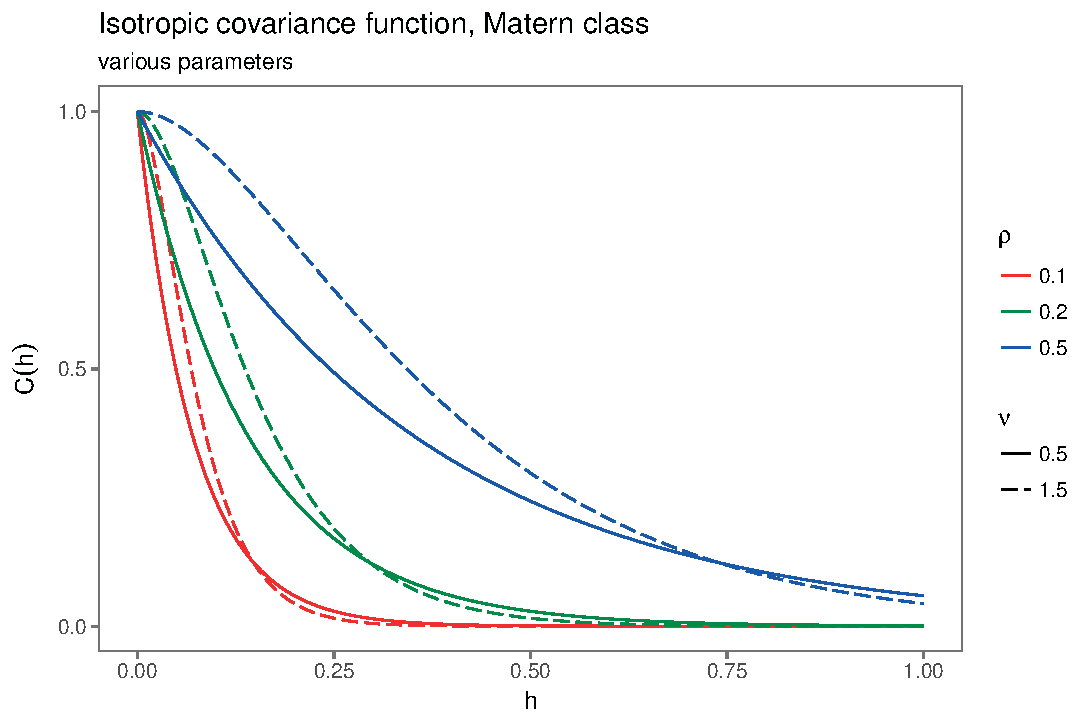
\includegraphics[width=0.95\textwidth]{matern_examples.pdf}
  \caption{\small The Mat\'ern isotropic covariance function \eqref{eq:matern} for various choices of $\nu$ and $\rho$, each with $\sigma^2 = 1$.}
  \label{fig:matern_examples}
\end{figure}


Another positive definite family, which we will use in examples below, is the \emph{exponentially damped cosine} class, 
\begin{equation} \label{eq:dampedcos}
  C(h) = \sigma^2 \exp \left( -\tau \frac{h}{\lambda} \right) \cos \left( \frac{h}{\lambda} \right), \qquad \tau \geq \frac{1}{\tan \frac{\pi}{2d}}, \quad \sigma^2,\lambda > 0.
\end{equation}
Unlike the Mat\'ern class, the damped cosine class allows for negative correlations at certain distances. This non-monotonic behavior is known in geostatistical applications as a \emph{hole effect}~\cite{Ye2015}, and is shown in Figure~\ref{fig:dampedcos_examples}. The restriction on $\tau$ that depends on $d$ is necessary for functions of this form to be positive definite. %Note, however, that $\tan(\pi/2d) \to 0$ as $d \to \infty$, so this set of functions is not a member of $\mathcal{C}_\infty$. 
The damped cosine family is not nearly as commonly used as the Mat\'ern family, but it is useful in some applications because allows for stochastically periodic behavior as well as negative correlations, which a Mat\'ern family cannot capture. However, it does not share the attractive feature of the Mat\'ern family that the smoothness of the process (i.e. the degree of differentiability) is controlled by a parameter that can be estimated from the data. The smoothness is closely related to the local behavior of the process, which crucial to obtaining good performance when interpolating the process at unobserved locations~\cite{Stein1999}.

\begin{figure}[!htb]
  \centering
  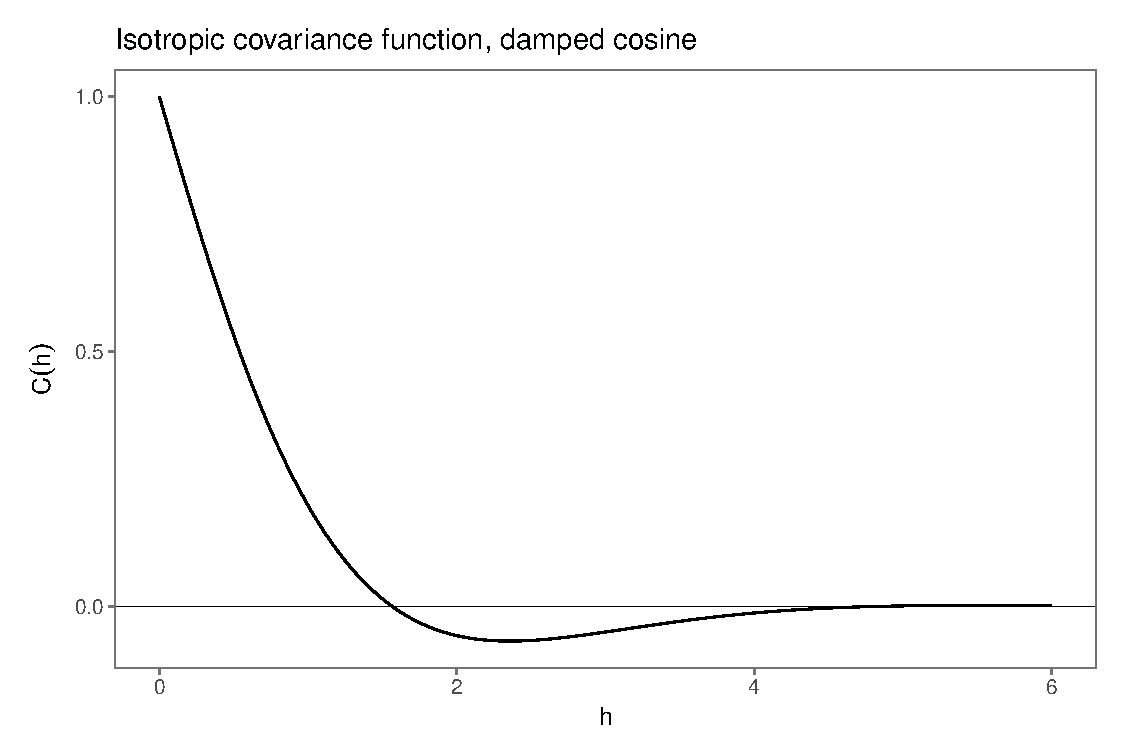
\includegraphics[width=0.95\textwidth]{dampedcos_examples.eps}
  \caption{\small The damped cosine isotropic covariance function \eqref{eq:dampedcos} for $\tau = 1$, $\lambda = 1$, and $\sigma^2=1$. Notice that $C(h) < 0$ for certain values of $h$.}
  \label{fig:dampedcos_examples}
\end{figure}

The strategy of fitting the data to a parametric family of covariance functions can produce a good estimate if the true covariance structure is close to the structure assumed by the choice of parametric family. However, there is no guarantee that this will be the case. For instance, if the true covariance contains a hole effect, there is no way for a Mat\'ern model to capture it since $C(h) > 0$ for all $h$. More preferable would be a flexible method that allows the spatial dependence in the data itself, rather than the choice of parametric family, to determine the shape of $C$.

% subsection estimating_the_covariance_function (end)

\subsection{The Spectral Domain and Bochner's Theorem} % (fold)
\label{sec:bochner_s_theorem}

The method proposed in this work takes advantage of the result from Bochner~\cite{bochner1955harmonic} which says that a real-valued continuous function $C$ is positive definite if and only if it is the Fourier transform of a symmetric, non-negative, finite measure $F$ on $\mathbb{R}^d$. That is, $C$ is positive definite if and only if
\begin{equation} \label{eq:bochner}
C(\bm{h}) = \int_{\mathbb{R}^d} \exp(i \bm{h}^T \bm{\omega}) \; dF(\bm{\omega}).
\end{equation}
In most circumstances, the measure $F$ has a Lebesgue density $f(\bm{\omega})$, which is referred to as the \emph{spectral density}~\cite{gelfand2010handbook}.  Furthermore, because we are assuming that the Gaussian process described by $C$ is isotropic, $C$ is a function of a scalar $h$, so that
\begin{equation} \label{eq:bochner2}
C(h) = \int_{\mathbb{R}} \cos(h\omega) \; f(\omega) \; d\omega.
\end{equation}
Stein~\cite{Stein1999} argues that for Gaussian process covariance functions to be realistic models for spatial phenomena, spectral densities $f(\omega)$ must be heavy tailed.

The relationship between the covariance function and the spectral density given in \eqref{eq:bochner2} suggests an alternative way to estimate the covariance function $C(h)$. If we can estimate the the symmetric spectral density $f(\omega)$, then we are assured that the corresponding covariance function $C(h)$ is positive definite.  Flexibly modeling $C(h)$ directly is difficult because of the restriction of positive definiteness, but flexibly modeling $f(\omega) $ is easy because it can be any symmetric density.

There have been previous approaches for non- and semi-parametric methods that estimate $C(h)$ using the spectral domain. Most closely related to our approach is that of Im, Stein, and Zhu~\cite{IM2007}, who estimate the spectral density using a combination of cubic B-splines with an explicitly specified algebraically decaying tail.   Constraints are placed on the spline coefficients to ensure that the spectral density is non-negative, thereby resulting in a covariance function is positive definite.  Im, Stein, and Zhu use the fact that when under isotropy, \eqref{eq:bochner} can be written as an integral over only one dimension,
\[
  C(h) = 2^{(d-2)/2}\Gamma(d/2) \int_0^\infty (hu)^{-(d-2)/2} J_{(d-2)/2}(hu) \; dG(u),
\]
where $J_\nu(\cdot)$ is the Bessel function of the first kind of order $\nu$. The spline-based spectral density is transformed into a covariance function using numerical integration, which is then used to construct the likelihood of the spline coefficients given the data.  This likelihood is be maximized over the constrained set of spline coefficients to produce $d\hat{G}(u)$, and hence $\hat{C}(h)$.  Our method follows this same concept, with some notable differences outlined in Section~\ref{section2:Procedure}.

Another, earlier method was put forth by Hall, Fisher and Hoffmann~\cite{Hall1994}. They proposed a multistep process which begins with a kernel estimate of the covariogram. Because the kernel estimate is not necessarily positive definite, they numerically compute its Fourier transform, set all frequencies beyond the first negative value to zero, and then numerically Fourier transform it back to the spatial domain. In the simulation study in Section~\ref{section3:Simulation-Study}, we compare our method to the one from Hall et al., as well as to the Mat\'ern model fit by maximum likelihood.

In Section~\ref{section4:Data-Application}, we apply our method to data from a paper by Singh et al. \cite{Singh2014}, where we model the thickness of a thin film semiconductor in a photovoltaic cell as a Gaussian process. The results are discussed in Section~\ref{section5:Conclusions}, as well as possibilities for improvements and future directions for this work.

% section bochner_s_theorem (end)


\section{Model and Estimation}
\label{section2:Procedure}

Throughout this section, assume that the data is observed at $n$ (not necessarily evenly spaced) spatial locations $\{\bm{s}_1, \dots, \bm{s}_n\}$. These locations exist on some bounded domain $\mathcal{D} \subseteq  \mathbb{R}^d$. The data, $\bm{y} =(y_1, \dots, y_n)^T$, is a realization of the random vector $\bm{Y} = (Y(\bm{s}_1), \dots, Y(\bm{s}_n))^T$, which constitute observations of single instance of a Gaussian process with mean 0 and stationary isotropic covariance function $C(h)$. %Then
% \[
%   \bm{Y} \sim \mathcal{N}_n(\bm{0}, \bm{\Sigma}),
% \]
% where $\Sigma_{ij} = C(|| \bm{s}_i - \bm{s}_j ||)$.  
We aim to estimate the covariance function.

\subsection{Estimating the Covariance Function} % (fold)
\label{sec:estimating_the_covariance_function}

Under the assumptions of stationarity and isotropy, the random vector $\bm{Y} \sim \mathcal{N}_n(\bm{0}, \bm{\Sigma})$, where the $ij$th element of $\bm{\Sigma}$ is
\[
  \Sigma_{ij} = \textrm{Cov}(y_i, y_j) = C(||\bm{s}_i - \bm{s}_j||) = C(h_{ij}).
\]
The scalar $h_{ij}$ is the Euclidean distance between locations $\bm{s}_i$ and $\bm{s}_j$. We can use \eqref{eq:bochner2} to obtain an integral representation for each element of $\bm{\Sigma}$,
\begin{equation} \label{eq:cov-elements-spectral}
  \Sigma_{ij} = \int \cos(h_{ij}\omega) \; f(\omega) \; d\omega.
\end{equation}
Rather than model the covariance function directly, we will model the spectral density with a semiparametric Bayesian model and use \eqref{eq:cov-elements-spectral} to construct the data likelihood.

% Were we able to sample from the spectral density $f(\omega)$, we could estimate $\Sigma_{ij}$ using Monte Carlo integration:
% \begin{equation}
%   \Sigma_{ij} \approx \widehat{\Sigma}_{ij} = \frac{1}{M} \sum_{m=1}^M \cos(h_{ij}\widetilde{\omega}_m)
% \end{equation}
% for $M$ samples $\{\widetilde{\omega}_1, \dots, \widetilde{\omega}_M\}$ from $f(\omega)$. The next section discusses an approach for approximating $f(\omega)$.

% section estimating_the_covariance_function (end)


\subsection{Calculating the Likelihood} % (fold)
\label{sec:calculating_the_likelihood}

Consider a rich family of spectral densities $f_{\bm{\theta}}(\omega)$ indexed by a parameter vector $\bm{\theta}$.  Since $\bm{Y} \sim \mathcal{N}_n(\bm{0}, \bm{\Sigma})$, the likelihood of $\bm{\theta}$ given the data $\bm{y}$ is
\begin{equation} \label{eq:loglik}
  \ell(\bm{\theta}; \bm{y}) = -\frac{n}{2} \log(2\pi) - \frac{1}{2} \log |\bm{\Sigma}(\bm{\theta})| - \frac{1}{2} \bm{y}^T \bm{\Sigma}(\bm{\theta})^{-1} \bm{y},
\end{equation}
where $\bm{\Sigma}(\bm{\theta})$ is defined as in \eqref{eq:cov-elements-spectral}.  In general, the solution to the Fourier transform integral in \eqref{eq:cov-elements-spectral} will not be available analytically.

Our strategy is to replace each element $\Sigma_{ij}(\bm{\theta})$ with a simple Monte Carlo approximation.  Suppressing dependence on $\bm{\theta}$ for notational convenience, we will use  
\begin{equation}
  \Sigma_{ij} = \int \cos(h_{ij}\omega) \; f(\omega) \; d\omega \approx  \frac{1}{M} \sum_{m=1}^M \cos(h_{ij}\widetilde{\omega}_m) = \widehat{\Sigma}_{ij},
\end{equation}
where $\widetilde{\omega}_1, \dots, \widetilde{\omega}_M$ are $M$ samples from $f_{\bm{\theta}}(\omega)$. We then plug $\widehat{\bm{\Sigma}}$ into the likelihood \eqref{eq:loglik} to estimate $\bm{\theta}$.


It is natural to ask how closely the likelihood evaluated using \eqref{eq:cov-elements-spectral} approximates the true likelihood.  The following theoretical result shows that the estimated likelihood $\hat{\ell}(\bm{\theta}; \bm{y})$ converges to the true likelihood $\ell(\bm{\theta}; \bm{y})$ almost surely as the number of Monte Carlo samples approaches infinity, even when the spectral density has heavy tails. A proof is given in the Appendix.

\begin{theorem}
  \label{thm:conssitency}
  Let $\bm{y} = (y_1, \dots, y_n)^T$ be a vector of observations from a mean-zero stationary, isotropic Gaussian process with covariance function $C(h)$, taken at locations $\bm{s}_1, \dots, \bm{s}_n \in \mathcal{D} \subseteq \mathbb{R}^d$ in some bounded domain $\mathcal{D}$.  For some symmetric density $f(\omega)$, let $\ell(\bm{y})$ be the likelihood
  \[
    \ell(\bm{y}) = -\frac{n}{2} \log(2\pi) - \frac{1}{2} \log(|\bm{\Sigma}|) - \frac{1}{2} \bm{y}^T \bm{\Sigma}^{-1} \bm{y},
  \]
where $\Sigma_{ij} = \int \cos(h_{ij}\omega)f(\omega)d\omega$, and $\hat{\ell}(\bm{y})$ be the Monte Carlo approximated likelihood
    \[
    \hat{\ell}(\bm{y}) = -\frac{n}{2} \log(2\pi) - \frac{1}{2} \log (| \widehat{\bm{\Sigma}}|) - \frac{1}{2} \bm{y}^T \widehat{\bm{\Sigma}}^{-1} \bm{y}
  \] 
where $\widehat{\Sigma}_{ij} = \frac{1}{M} \sum_{m=1}^M \cos(\widetilde{\omega}_m h_{ij})$, and $\widehat{\omega}_1, \dots, \widehat{\omega}_M$ are an iid sample from $f(\omega)$.  Then as $M \to \infty$,
\[
\hat{\ell}(\bm{y}) \to \ell(\bm{y}) \text{ a.s.-}f_\omega.
\]

    
%     Then the distribution of $\bm{Y}$ is
%   \[
%     \bm{Y} \sim \mathcal{N}_n(0, \bm{\Sigma})
%   \]
%   where $\Sigma_{ij} = C(||\bm{s}_i - \bm{s}_j||) = C(h_{ij})$. The true likelihood function is
%   \[
%     \ell(\bm{\Sigma}; \bm{y}) = -\frac{n}{2} \log(2\pi) - \frac{1}{2} \log \det (\bm{\Sigma}) - \frac{1}{2} \bm{y}^T \bm{\Sigma}^{-1} \bm{y}.
%   \]
%   Suppose we observe data $\bm{y} = (y_1, \dots, y_n)^T$ from this Gaussian process. Let
%   \[
%     \hat{\ell}(\widehat{\bm{\Sigma}}; \bm{y}) = -\frac{n}{2} \log(2\pi) - \frac{1}{2} \log \det (\widehat{\bm{\Sigma}}(\bm{\beta})) - \frac{1}{2} \bm{y}^T \widehat{\bm{\Sigma}}^{-1}(\bm{\beta}) \bm{y}
%   \]
%   be the approximated likelihood from our proposed method. The $(i,j)$th element of the approximated covariance matrix $\widehat{\bm{\Sigma}}$ is defined as
%   \[
%     \widehat{\Sigma}_{ij} = \frac{1}{M} \sum_{m=1}^M \cos(\widetilde{\omega}_m h_{ij})
%   \]
%   where $\{\widehat{\omega}_1, \dots, \widehat{\omega}_M\}$ are random samples distributed according to the spectral density $f_\omega$. Then as $M \to \infty$, $\hat{\ell}(\bm{\beta}; \bm{y}) \to \ell(\bm{\Sigma}; \bm{y})$ a.s. $f_\omega$.
\end{theorem}

Theorem \ref{thm:conssitency} says that as long as we are willing to draw a large enough collection of Monte Carlo samples from a spectral density $f_{\bm{\theta}}(\omega)$, the Monte Carlo estimated likelihood of $\bm{\theta}$ will get arbitrarily close to the exact likelihood.  Furthermore, this remains true even when $f_{\bm{\theta}}(\omega)$ has heavy tails, as we expect for realistic models of spatial phenomena.




% To be explicit, in \eqref{eq:loglik} the estimated covariance matrix $\widehat{\bm{\Sigma}}$ is expressed as a function of $\bm{\beta}$ because
% \[
%   \widehat{\Sigma}_{ij} = \frac{1}{M} \sum_{m=1}^M \cos(h_{ij} \widetilde{\omega}_m),
% \]
% \[
%   \widetilde{\omega}_m \overset{\textrm{i.i.d.}}{\sim} \hat{f}(\omega),
% \]
% and
% \[
%   \log \hat{f}(\log \omega) = \sum_{k=1}^K \beta_k B_k(\log \omega).
% \]
% The only free parameters in this procedure are the values of $\bm{\beta}$. This is summarized in Algorithm~\ref{alg:lik}.

% From \eqref{eq:spline}, we can transform back to $\hat{f}(\omega)$, integrate numerically, and sample via the inverse CDF method.

% \begin{algorithm}[!htb]
%   \caption{\small Calculating the log likelihood} \label{alg:lik}
%   \begin{algorithmic}[1]
%     \Procedure{Likelihood}{$\bm{\beta}, \bm{y}$}
%     \State $\log \hat{f}(\log \omega) = \sum_{k=1}^K \beta_k B_k(\log \omega)$\Comment{$k$ preselected knot locations}
%     \State Sample $\widetilde{\omega}_1, \dots, \widetilde{\omega}_M$ from $\hat{f}(\omega)$\Comment{Inverse CDF method; $M$ large}
%     \For{$1 \leq i,j \leq n$}
%       \State $\widehat{\Sigma}_{ij} = \frac{1}{M} \sum_{m=1}^M \cos(h_{ij} \widetilde{\omega}_m)$\Comment{$h_{ij}$: distance between locations $\bm{s}_i$ and $\bm{s}_j$}
%     \EndFor
%     \State $\hat{\ell}(\bm{\beta}; \bm{y}) = -\frac{n}{2} \log(2\pi) - \frac{1}{2} \log |\widehat{\bm{\Sigma}}| - \frac{1}{2} \bm{y}^T \widehat{\bm{\Sigma}}^{-1} \bm{y}$
%     \EndProcedure
%   \end{algorithmic}
% \end{algorithm}





















\subsection{Semiparametric Modeling of the Spectral \\ Density} % (fold)
\label{sec:semiparametric_modeling_of_the_spectral_density}

Since we don't want to impose a parametric form for $f(\omega)$, we will model it semiparametrically using splines. According to Bochner's theorem, $f(\omega)$ is a symmetric density, so it suffices to restrict our attention to modeling $f(\omega)$ for $\omega > 0$.

Rather than modeling $f(\omega)$ directly, we apply a straightforward variable transformation and model $\log f(\log \omega)$ instead. Working on the log-log scale is a natural way to flexibly specify densities with heavy tails.  It is easy to show that any density with power law tails has linear tails on the log-log scale. Suppose $f_X(x) = cx^{-b}$, $b > 1$, and let $Y = \log X$. Then
\begin{align*}
  f_Y(y) &= f_X(e^y) \frac{d}{dy}(e^y) \\
  &= ce^{-by}e^y \\
  &= ce^{-(b-1)y},
\end{align*}
and so
\[
  \log f_Y(y) \propto -(b-1)y.
\]
This fact is illustrated further in Figure~\ref{fig:logdens_ex}.

\begin{figure}[!htb]
  \centering
  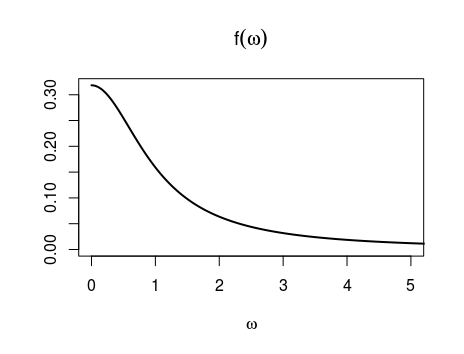
\includegraphics[width=0.48\textwidth]{dens_ex.png}
  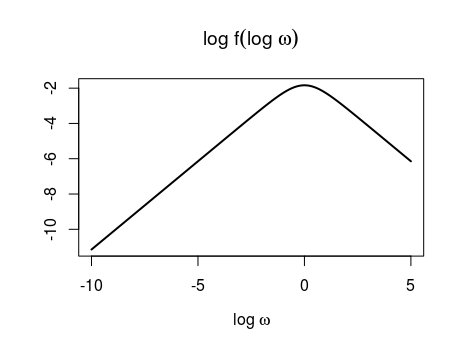
\includegraphics[width=0.48\textwidth]{logdens_ex.png}
  \caption{\small A density $f(\omega)$ with power law tails (left) and the same density transformed to the log-log scale (right). Both the left and right tails of the transformed density are linear.}
  \label{fig:logdens_ex}
\end{figure}

An important benefit to working in this log-transformed space is that linear tails are ideal for modeling the curve using a natural spline basis, which is constructed to ensure linearity beyond the outermost (\emph{boundary}) knots. If we are willing to assume that the tails of $\log f(\log \omega)$ are truly linear, then fitting it with natural splines will result in a good approximation over then entire domain $\log \omega \in (-\infty, \infty)$ without needing to use a large number of basis functions.

It might appear that requiring that $f(\omega)$ have power law tails is more restrictive than we would like. After all, the goal is to avoid the need to restrict $C(h)$ to a particular parametric family. However, the class of covariance functions that result from the Fourier transform of power law spectral densities is significantly broader than any of the parametric families, yet Bochner's theorem still guarantees that they are positive definite. In fact, this class covers most covariance models of practical interest, including the entire Mat\'ern class with finite $\nu$. Gaussian processes with spectral densities that decay quickly, e.g. with exponential tails, yield realizations that are generally regarded as unrealistically smooth~\cite{Stein1999}. %Two spatial locations a moderate distance apart would have nearly zero covariance, which is not an acceptably accurate model for real spatial data. By exclusively working with spectral densities that decay more slowly, we are restricting ourselves to the more realistic scenario where two locations can be far apart but still have a non-negligible covariance between them.

To model $\log f(\log \omega)$ using natural cubic splines, let
\begin{equation} \label{eq:spline}
  \log f(\log \omega) = \sum_{k=1}^K \beta_k B_k(\log \omega),
\end{equation}
where $\bm{\beta} = (\beta_1, \dots, \beta_K)^T$ are coefficients associated with $K$ known cubic spline basis functions $B_1(\cdot), \dots, B_K(\cdot)$. The $K$ basis functions are centered around a collection of $K$ locations referred to as knots.

% section semiparametric_modeling_of_the_spectral_density (end)

% section calculating_the_likelihood (end)

\subsection{Estimating the Spline Coefficients} % (fold)
\label{sec:estimating_the_spline_coefficients}


For a given collection of basis functions, the likelihood of the parameter vector $\bm{\theta} = \bm{\beta} = (\beta_1, \dots, \beta_K)^T$ can be approximated by plugging \eqref{eq:cov-elements-spectral} into \eqref{eq:loglik}. To be explicit, in \eqref{eq:loglik} the estimated covariance matrix $\bm{\Sigma}$ is expressed as a function of $\bm{\beta}$ because
\[
  \Sigma_{ij} = \int \cos(h_{ij}\omega) \, f_{\bm{\beta}}(\omega) \, d\omega \approx  \frac{1}{M} \sum_{m=1}^M \cos(h_{ij} \widetilde{\omega}_m) = \widehat{\Sigma}_{ij},
\]
\[
  \widetilde{\omega}_m \overset{\textrm{i.i.d.}}{\sim} f_{\bm{\beta}}(\omega),
\]
and
\[
  \log f_{\bm{\beta}}(\log \omega) = \sum_{k=1}^K \beta_k B_k(\log \omega).
\]
The only free parameters in this procedure are the elements of $\bm{\beta}$. This is summarized in Algorithm~\ref{alg:lik}.

To quickly generate the samples $\widetilde{\omega}_1, \ldots, \widetilde{\omega}_M$, we transform $\log f_{\bm{\beta}}(\log \omega)$ back to $f_{\bm{\beta}}(\omega)$, integrate numerically, and sample via the inverse CDF method.

\begin{algorithm}[!htb]
  \caption{\small Calculating the log likelihood $\hat{\ell}(\bm{\beta}; \bm{y})$} \label{alg:lik}
  \begin{algorithmic}[1]
    \Procedure{Likelihood}{$\bm{\beta}, \bm{y}$}
    \State $\log f_{\bm{\beta}}(\log \omega) = \sum_{k=1}^K \beta_k B_k(\log \omega)$\Comment{$k$ preselected knot locations}
    \State Sample $\widetilde{\omega}_1, \dots, \widetilde{\omega}_M$ from $f_{\bm{\beta}}(\omega)$\Comment{Inverse CDF method; $M$ large}
    \For{$1 \leq i,j \leq n$}
      \State $\widehat{\Sigma}_{ij} = \frac{1}{M} \sum_{m=1}^M \cos(h_{ij} \widetilde{\omega}_m)$\Comment{$h_{ij}$: distance between locations $\bm{s}_i$ and $\bm{s}_j$}
    \EndFor
    \State $\hat{\ell}(\bm{\beta}; \bm{y}) = -\frac{n}{2} \log(2\pi) - \frac{1}{2} \log |\widehat{\bm{\Sigma}}| - \frac{1}{2} \bm{y}^T \widehat{\bm{\Sigma}}^{-1} \bm{y}$
    \EndProcedure
  \end{algorithmic}
\end{algorithm}

Since we can calculate the likelihood as a function of the data and $\bm{\beta}$, we can estimate $\bm{\beta}$ using a Markov chain Monte Carlo (MCMC) algorithm. %However, the problem of choosing how many knots to use and where they should be located still remains.

To complete the model, we specify priors for $\bm{\beta}$ according to the Bayesian formulation of penalized splines introduced in~\cite{lang2004bayesian}.  The penalization corresponds to priors that specify to a second-order random walk, with
\[
  \beta_k \;|\; \tau^2 \sim \mathcal{N}(2\beta_{k-1} - \beta_{k-2}, \; \tau^2)
\]
where
\[
  \beta_2 \;|\; \tau^2 \sim \mathcal{N}(\beta_1, \; \tau^2)
\]
and
\[
  \beta_1 \;|\; \tau^2 \sim \mathcal{N}(0, \; \tau^2).
\]
The variance parameter $\tau^2$ controls the smoothness of the spline fit, and must also be estimated. Its prior is specified as
\[
  \tau^2 \sim \mathcal{N}^+(0, \; \sigma^2_\tau),
\]
the half-normal distribution with some variance hyperparameter $\sigma^2_\tau$.

With the priors specified, we can proceed with the MCMC algorithm in Algorithm~\ref{alg:mcmc}. We use a Metropolis-Hastings update to determine whether or not to accept the joint proposal $\bm{\beta}$. The result is random draws from the posterior distribution of $\bm{\beta} \;|\; \bm{y}$.

\begin{algorithm}[!htb]
  \caption{\small Metropolis-Hastings Sampler} \label{alg:mcmc}
  \begin{algorithmic}[1]
    \Procedure{MCMC}{$\bm{\beta}, \bm{y}$}
    \State $\bm{\beta}_1 \gets \bm{\beta}$\Comment{Initialization}
    \For{$2 \leq i \leq N$}\Comment{$N$ large}
    \State Propose new $\bm{\beta}^* \sim q(\cdot)$
    \State $\ell_0 = \hat{\ell}(\bm{\beta}_{i-1}, \bm{y})$\Comment{See Algorithm~\ref{alg:lik}}
    \State $\ell_1 = \hat{\ell}(\bm{\beta}^*, \bm{y})$
    \State $a = \Big[\pi(\bm{\beta}^*) \cdot \ell_1 \cdot q(\bm{\beta}_{i-1}|\bm{\beta}^*)\Big]/\Big[\pi(\bm{\beta}_{i-1}) \cdot \ell_0 \cdot q(\bm{\beta}^*|\bm{\beta}_{i-1})\Big]$
    \State Generate $u \sim Unif(0, 1)$
    \If{$u < \min(a, 1)$}
    \State $\bm{\beta}_i \gets \bm{\beta}^*$\Comment{Accept the proposal}
    \Else
    \State $\bm{\beta}_i \gets \bm{\beta}_{i-1}$\Comment{Reject the proposal}
    \EndIf
    \EndFor
    \EndProcedure
  \end{algorithmic}
\end{algorithm} 



% section estimating_the_spline_coefficients (end)

\subsection{Computational Challenges} % (fold)
\label{sec:computational_challenges}

The primary difficulty inherent in this method is that it is extraordinarily computationally intensive, requiring a Monte Carlo approximation for every element of the covariance matrix. For a moderately large number of observations, say $n = 400$, we need to estimate $\frac{n(n-1)}{2} = 79800$ separate elements. For each of these elements, we need to perform a Monte Carlo integration with a large number of samples. This all happens within one likelihood calculation, and we need to compute the likelihood at every iteration of the MCMC algorithm. The computational costs would be prohibitive for a na\"{i}ve implementation of this method.

Fortunately, most of these difficulties can be assuaged by taking advantage of parallel computing. Algorithm~\ref{alg:mcmc} requires previous information $\bm{\beta}_{i-1}$ to compute $\bm{\beta}_i$, so unfortunately it would be extremely difficult to restructure it in a way where multiple updates are being performed simultaneously. However, it is possible to parallelize aspects of the likelihood calculation in Algorithm~\ref{alg:lik}.

Consider the \textbf{for} loop in Algorithm~\ref{alg:lik}. For each value of $i$ and $j$, the computation of
\[
  \widehat{\Sigma}_{ij} = \frac{1}{M} \sum_{m=1}^M \cos(h_{ij} \widetilde{\omega}_m)
\]
depends on two values: $h_{ij}$, the distance between $\bm{s}_i$ and $\bm{s}_j$, and $\widetilde{\bm{\omega}}$, the vector of $M$ samples from $f(\omega)$. It does not depend on any previously computed element of $\widehat{\bm{\Sigma}}$. Therefore, performance would improve dramatically if we could calculate the estimates simultaneously, in parallel.

There are several options for speeding up a parallelizable problem. The simplest, and least reliant on expensive additional hardware, is \emph{parallel processing}~\cite{suchard2010understanding}. Today, most personal computers ship with CPUs that contain 2, 4, or even 8 computing cores. Each core is capable of running a single set of sequential instructions. By using tools such as OpenMP, users can write code that will assign a set of instructions to every available core. The instructions will execute simultaneously, and the results are gathered together upon completion. Of course, the potential speedup is limited by the number of cores available in the CPU---if there are 4 cores, the instructions will be executed in about one fourth of the time.

This type of parallel processing works well for problems like obtaining multiple MCMC chains at the same time. For the estimation of $\bm{\Sigma}$ in this context, however, it is not optimal. Recall that for $n = 400$, we need to estimate $79800$ elements of $\bm{\Sigma}$. Reducing this by a factor of 4 is helpful, but ideally we would like to perform all $79800$ at once, not just take them four at a time.

Another option is to utilize a computing cluster. Clusters usually are large rooms filled with racks of computers, connected in such a way that one process can be spread uniformly across them and use hundreds or thousands of cores at once~\cite{suchard2010understanding}. One downside to this approach is that access to such a cluster is difficult to get, outside of a large company or academic institution. Beyond that, though, latency starts to become a problem when dealing with clusters. Because the cores are spread over many physical computers, the increases in computational speed becomes overwhelmed by the large amount of time it takes to share data between the cores. As a result, the overall performance increase may not be as large as we might expect.

A third option is \emph{GPU computing}. Originally created to run video games, graphics processing units, or GPUs, have become increasingly popular for parallel computing. CPUs contain a small number of cores that are optimized to handle highly complex instructions quickly. By contrast, GPUs are made up of thousands of simple, highly efficient cores that are optimized for simpler instructions and designed to work in parallel with each other. Because the GPU cores lack many of the sophisticated features of CPU cores (a sacrifice made in exchange for speed and efficient exchange of data), the programmer must have a more intricate knowledge of the architecture of their particular GPU in order to get the best possible speedup. Fortunately, directives such as OpenACC let the compiler make most of the architecture-related decisions instead of leaving them in the hands of the user.

To take full advantage of the highly parallelizable nature of the covariance estimation problem, I have chosen the GPU option. I wrote the code to carry out the Monte Carlo integrations in CUDA C. CUDA is an API provided by Nvidia that allows users to write programs in C or Fortran that interact with Nvidia brand GPUs. Computations were done on three different hardware setups:

\begin{itemize}
  \item Nvidia GeForce GTX 1060 GPU, on a personal computer running Ubuntu 16.04;
  \item Nvidia Tesla P100 GPU, provided by Penn State University's Institute for CyberScience Advanced CyberInfrastructure (ICS-ACI);
  \item Nvidia Tesla K80 GPU, running on an Amazon EC2 instance.
\end{itemize}

With these tools, the computations can be performed fairly quickly. On the Tesla P100, one entire likelihood calculation described by Algorithm~\ref{alg:lik} with $M = 50000$ and $N = 400$ completes in just under one second.

To illustrate the power of parallel computing, and to show that this element-wise approximation to the covariance matrix is a feasible approach, Figure~\ref{fig:timings-mc} shows the results of an experiment comparing the runtime of the Monte Carlo approximation from Algorithm~\ref{alg:lik} to the runtime of the exact covariance calculation. That is, for a fixed $N$, generate 100 sets of points $\bm{s}_1, \dots, \bm{s}_N$ and their distances $h_{ij} = ||\bm{s}_i - \bm{s}_j||$. Also generate $M = 20000$ samples $\widetilde{\omega}_1, \dots, \widetilde{\omega}_M$ from the spectral density $f(\omega)$ corresponding to a Mat\`ern covariance function. Since the computational cost of the random sample generation is constant regardless of $N$, it is not included when timing.
\[
  \Sigma_{ij} = C(h_{ij})
\]
and
\[
  \widehat{\Sigma}_{ij} = \frac{1}{M}\sum_{m=1}^M \cos(h_{ij} \widetilde{\omega}_{m})
\]
100 times each, and compare the median runtimes as a function of $N$.

Notice from Figure~\ref{fig:timings-mc} that for large enough $N$, it actually becomes faster to perform a Monte Carlo approximation to the elements of $\Sigma$ than to directly plug in the distances to the covariance function $C$. In this experiment $N$ needed to be greater than about 2000, but this is of course hardware dependent.

This is not a surprising result considering the parallelized nature of the Monte Carlo approximation. As $N$ increases, the exact calculation must handle all additional computations sequentially, whereas the Monte Carlo approximation can simply allocate more cores that execute their tasks simultaneously. As a result, the Monte Carlo runtime increases more slowly with $N$ than the exact covariance runtime.

However, there are nontrivial computational costs associated with GPU computing that cause it to be significantly slower than the exact alternative when $N$ is not large. In Figure~\ref{fig:timings-mc}, it appears that the Monte Carlo runtime is more or less unchanged from $N = 40$ to $N = 400$. The bottleneck here is data transfer and allocation. For small $N$, the time required to do the calculations themselves is negligible compared to the time required to allocate memory on the GPU, transfer the spectral density samples from the CPU to the GPU, combine the results, and transfer them back to the CPU. This is the reason that sometimes, seemingly paradoxically, parallelizing a routine can cause it to execute more slowly than the equivalent sequential routine. But for large enough $N$, we expect the speedup to be substantial.

\begin{figure}[htbp]
  \centering
  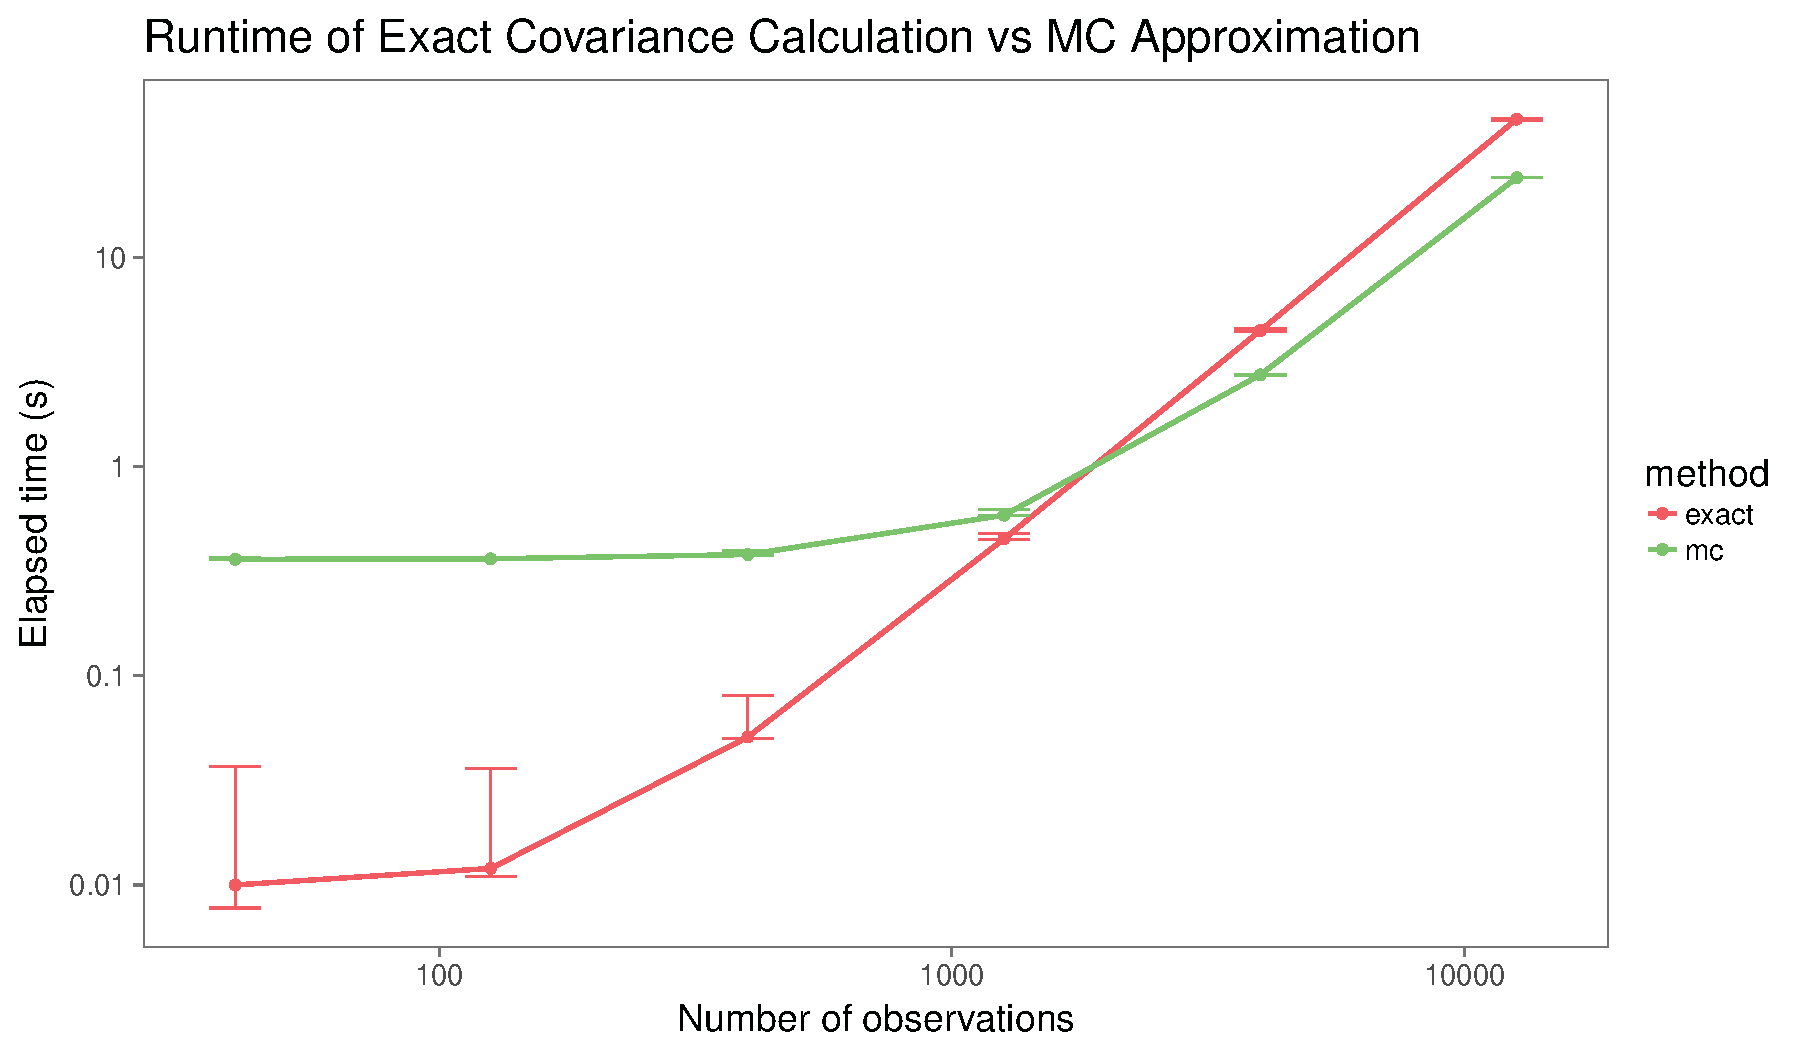
\includegraphics[width=0.95\textwidth]{timings_mc.pdf}
  \caption{Elapsed time taken to calculate the element-wise Monte Carlo approximation to the covariance matrix corresponding to a Mat\'ern covariance function, versus calculating it directly using $C(h)$. The covariance matrix is $n \times n$, where $n$ is the number of observations. Each method was run 100 times for every value of $n$. The medians are plotted with dots and connected with a line. The error bars represent the range from the first to third quartiles---some times for the exact calculation were misleadingly high due to CPU wakeup. GPU computations were done on a Tesla P100. Note the logarithmic axes.}
  \label{fig:timings-mc}
\end{figure}

% section computational_challenges (end)

\section{Simulation Study}
\label{section3:Simulation-Study}

In this section we will present some results that compare the method presented in Section~\ref{section2:Procedure}, which we will refer to as the ``spline method,'' to some existing techniques for estimating covariance functions. In Section~\ref{sec:comparing_exact_and_estimated_log_likelihoods}, we examine the accuracy of the likelihood estimate from Algorithm~\ref{alg:lik}. In Sections~\ref{sec:prediction_performance} and \ref{sec:covariance_function_estimation_performance}, we compare the spline method to existing methods with regard to prediction performance and how closely they estimate the true covariance function, respectively.

\subsection{Comparing Exact and Estimated Log Likelihoods} % (fold)
\label{sec:comparing_exact_and_estimated_log_likelihoods}

Assume we observe $\bm{y} = (y_1, \dots, y_{400})^T$ from a Gaussian process where the covariance function is Mat\'{e}rn (see \eqref{eq:matern}) with known parameters $\nu$, $\rho$, and $\sigma$. The observations come from locations $\bm{s}_1, \dots, \bm{s}_{400}$ spread randomly over the unit square in $\mathbb{R}^2$. Because we know $C(h)$, we can calculate the covariance matrix exactly:
\[
  \bm{\Sigma}_{ij} = C(||\bm{s}_i - \bm{s}_j||).
\]
From this we can find the exact likelihood.

The spectral density corresponding to the Mat\'{e}rn covariance function \eqref{eq:matern} is
\[
  f(\omega) = \frac{\sigma g(\nu, \rho)}{\big( \frac{4\nu}{\rho^2} + \omega^2 \big)^{\nu+d/2}},
\]
where $d = 2$ is the dimension of the spatial domain and
\[
  g(\nu, \rho) = \frac{\Gamma\left(\nu + \frac{d}{2}\right)(4\nu)^\nu}{\pi^{d/2} \rho^{2\nu} \Gamma(\nu)}.
\]
Because we can calculate the spectral density directly in this scenario, we can avoid fitting the splines and estimating $\bm{\beta}$. By bypassing this step, we test just the procedures for sampling from $f(\omega)$ and estimating the log likelihood.

To perform the test, we chose two values for $\nu$ and six values for $\rho$. The $\sigma^2$ parameter just controls the marginal variance $\textrm{Var}(\bm{Y}(\bm{s}))$, and so it can be factored out of the covariance matrix $\bm{\Sigma}$. For each combination of parameter settings, we generated 100 Gaussian process realizations and compared the true and estimated log likelihoods. The results are summarized in Figure~\ref{fig:liks_by_rho}. Note that the estimated likelihoods are close to their true values in all cases, and the choice of $\rho$ does not appear to significantly affect the accuracy.

\begin{figure}[!htb]
  \centering
  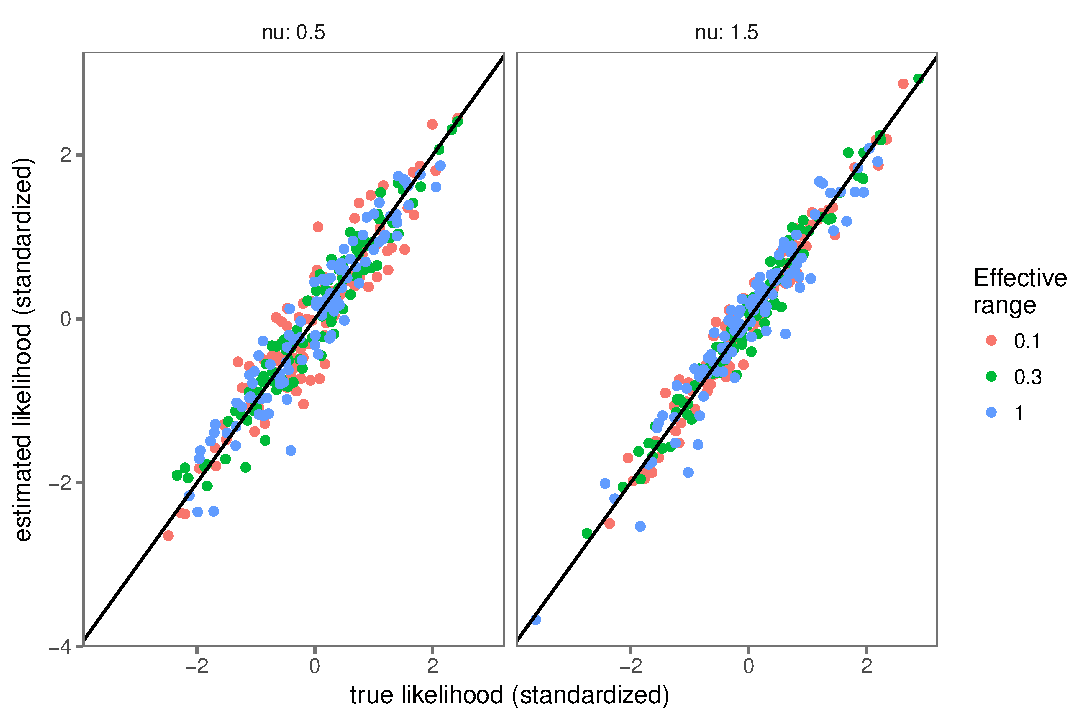
\includegraphics[width=0.95\textwidth]{lik_true_vs_est.pdf}
  \caption{\small Comparing true and estimated log likelihoods for varying values of $\rho$ (given above each plot). Values in each plot were centered and scaled for easier comparison. The likelihoods for the two values of $\nu$, $0.5$ and $1.5$, yield a similar pattern.}
  \label{fig:liks_by_rho}
\end{figure}

% \begin{figure}[htbp]
%   \centering
%   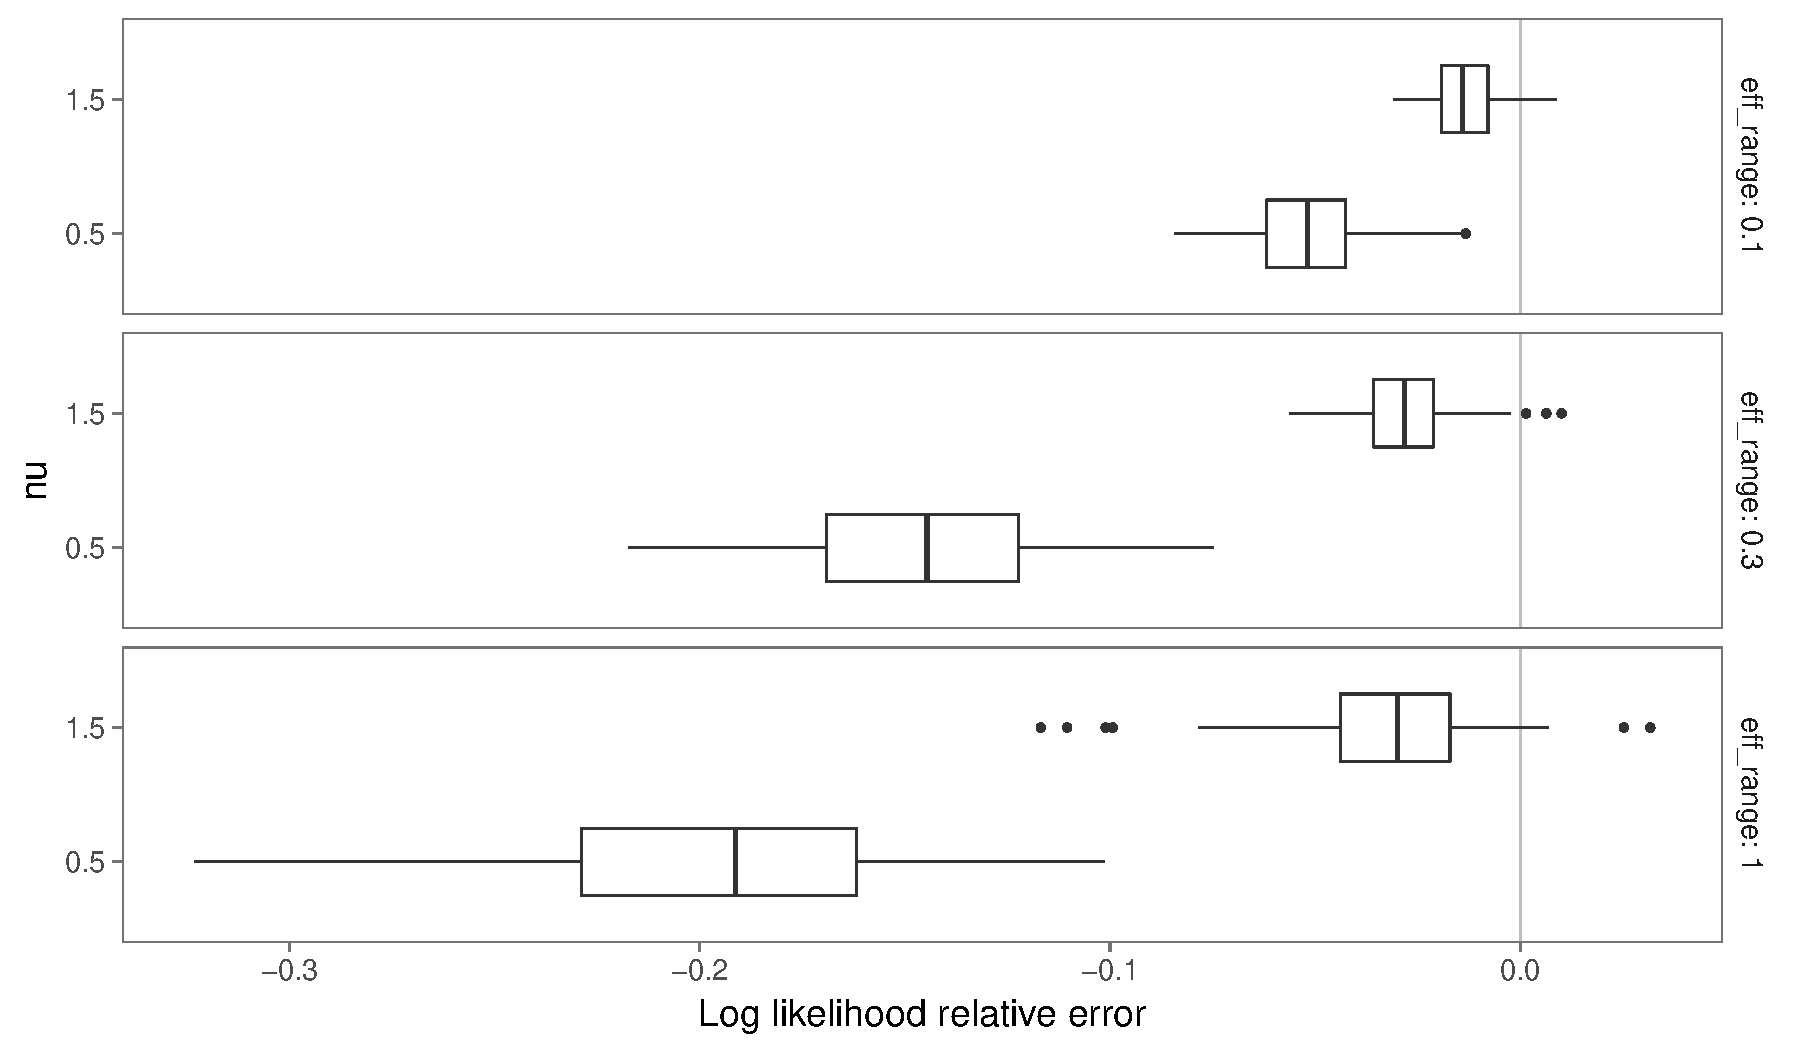
\includegraphics[width=0.95\textwidth]{rel_ll_err_1.pdf}
%   \caption{Relative error of the estimated log likelihood. Samples came directly from the true spectral density $f(\omega)$. Each facet of the plot corresponds to different effective ranges (0.1, 0.3, 1), and contains a boxplot for each of $\nu = 0.5$ and $\nu = 1.5$. Every boxplot is made from 100 different datasets.}
%   \label{fig:rel-ll-err-1}
% \end{figure}

We ran a second version of this test that incorporated the $\bm{\beta}$ estimation. Still assuming the true $f(\omega)$ is known, we took 50 equally spaced points along $\log f(\log \omega)$ and fit natural splines to those points. This gave us some $\bm{\beta}_{\textrm{opt}}$, the values for $\bm{\beta}$ that most closely approximate $\log f(\log \omega)$. Then using $\bm{\beta}_{\textrm{opt}}$ we estimated the likelihood and again compared it to the true likelihood. Results are shown in Figure~\ref{fig:estliks_spline_rho}. The estimated likelihoods are still comparable to their true values, despite the fact that we are sampling from a spline approximation to $f(\omega)$ rather than $f(\omega)$ itself.

\begin{figure}[!htb]
  \centering
  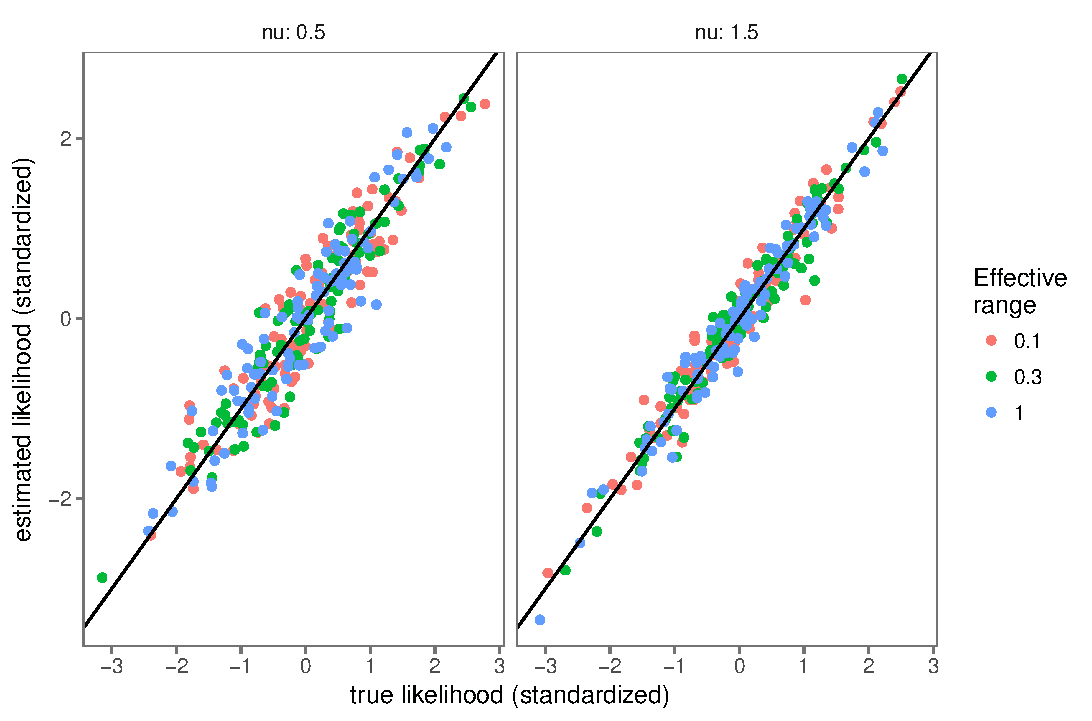
\includegraphics[width=0.95\textwidth]{lik_true_vs_est2.pdf}
  \caption{\small Comparing true and estimated log likelihoods for varying values of $\rho$ (given above each plot). Unlike the results in Figure~\ref{fig:liks_by_rho}, these estimates were generated not by sampling from $f(\omega)$ directly, but by sampling from a density approximating $f(\omega)$ fit using splines.}
  \label{fig:estliks_spline_rho}
\end{figure}

% \begin{figure}[htbp]
%   \centering
%   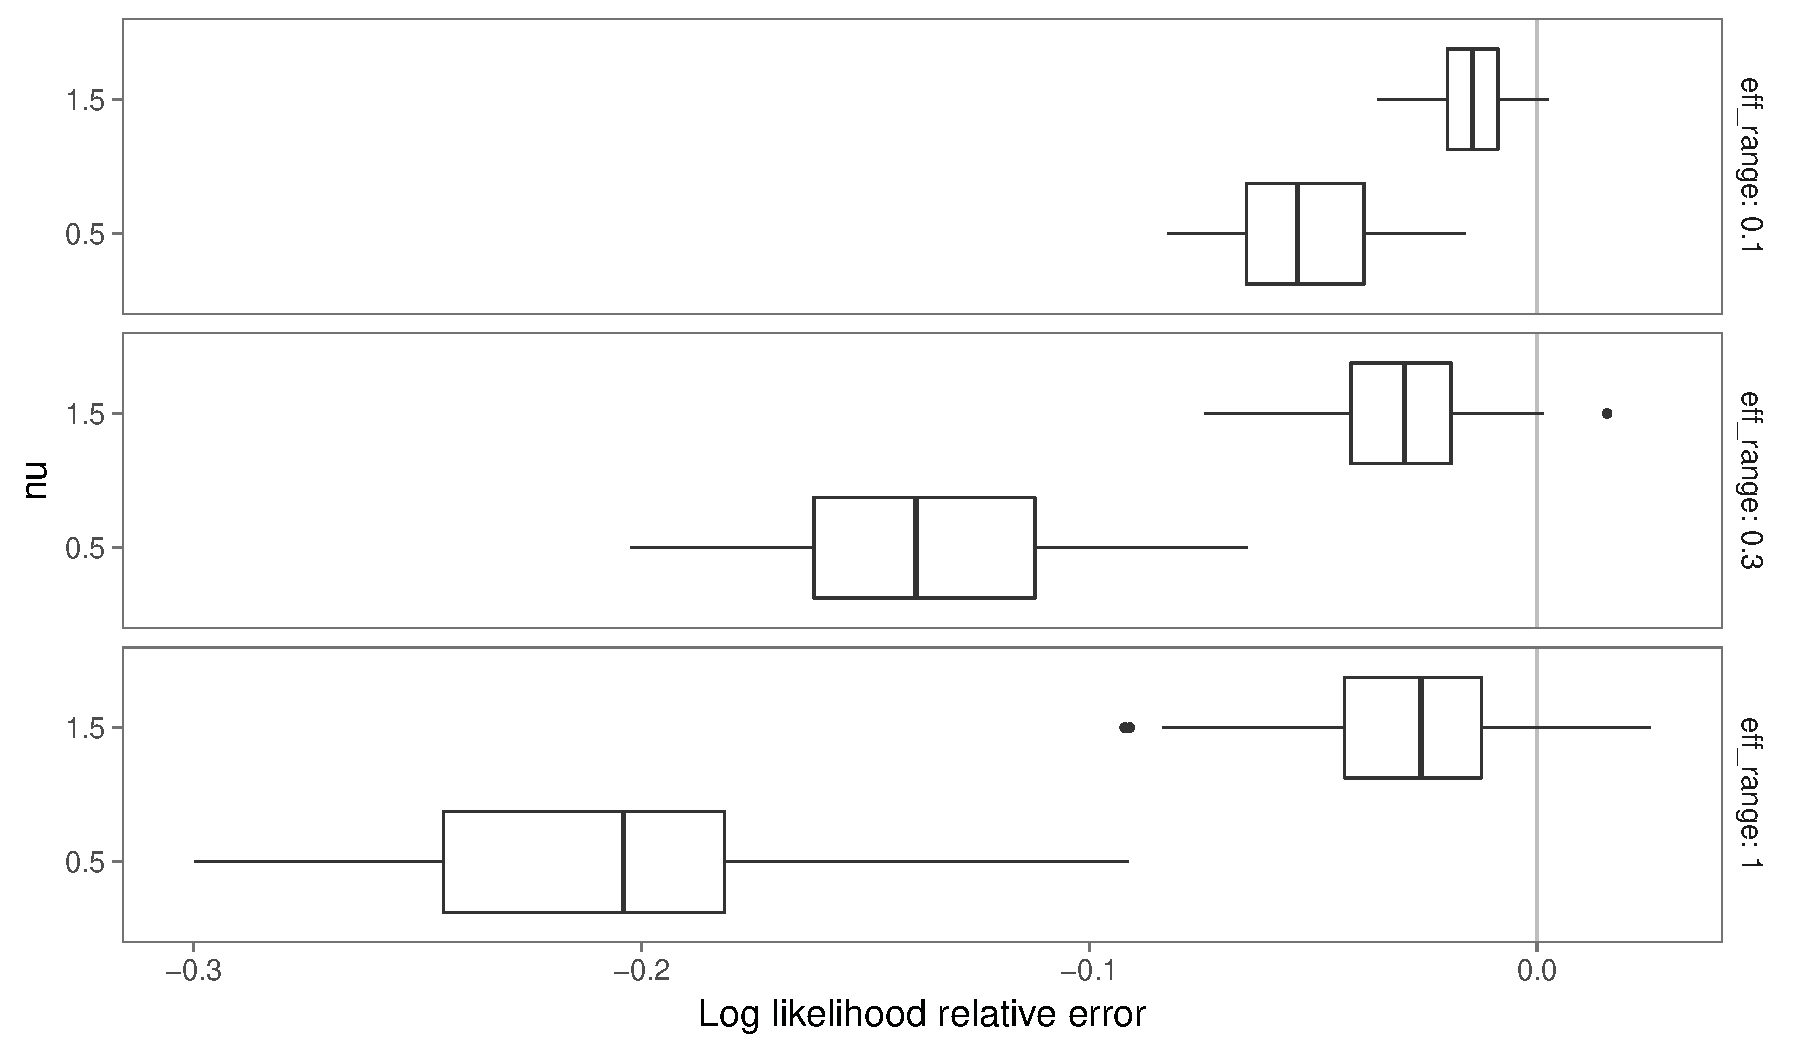
\includegraphics[width=0.95\textwidth]{rel_ll_err_2.pdf}
%   \caption{Relative error of the estimated log likelihood. Unlike the results in Figure~\ref{fig:liks_by_rho}, these estimates were generated not by sampling from $f(\omega)$ directly, but by sampling from a density approximating $f(\omega)$ fit using splines. Each facet of the plot corresponds to different effective ranges (0.1, 0.3, 1), and contains a boxplot for each of $\nu = 0.5$ and $\nu = 1.5$. Every boxplot is made from 100 different datasets.}
%   \label{fig:rel-ll-err-2}
% \end{figure}

\begin{figure}[htbp]
  \centering
  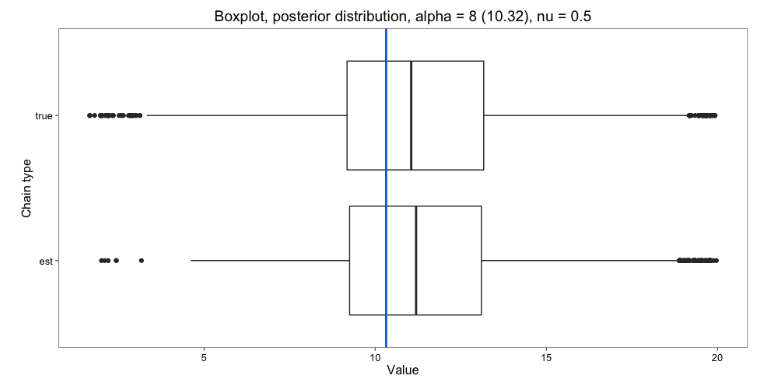
\includegraphics[width=0.95\textwidth]{est_vs_true_8_0-5_2.png}
  \caption{Posterior distributions of $\rho|\bm{y}$ for the true likelihood function and our estimated likelihood. This plot shows $\alpha$, which occurs in another parameterization of the Mat\'ern covariance function and is simply $1/\rho$. The observations were simulated with a value of $\alpha = 8$, but the maximum likelihood estimate given the data was $\hat{\alpha}_{MLE} = 10.32$.}
  \label{fig:compare-one}
\end{figure}

As an additional test that we are correctly estimating the true likelihood, we simulated another set of 400 observations $\bm{y} = (y_1, \dots, y_{400})^T$ from a Gaussian process with Mat\'ern covariance function. We treat $\rho$ and $\nu$ as fixed and known, and used MCMC to find the posterior distribution of $\rho|\bm{y}$ using the true likelihood function, and again using the estimated likelihood from Algorithm~\ref{alg:lik}. One result from this test is shown in Figure~\ref{fig:compare-one}. We see that the two posterior distributions are very similar, futher indicating that our likelihood estimate is reasonable for use in our more complicated semiparametric MCMC (Algorithm~\ref{alg:mcmc}).

\subsection{Prediction Performance} % (fold)
\label{sec:prediction_performance}

Next, we put the entire procedure from Algorithm~\ref{alg:mcmc} into motion. First, $n = 400$ observations $\bm{y} = (y_1, \dots, y_{400})^T$ are drawn from a Gaussian process with a Mat\`{e}rn covariance function with $\nu = 1.5$, $\rho = 0.1548$, and $\sigma = 1$. This particular value of $\rho$ was chosen to obtain an effective range of 0.3. The observation locations are randomly spread across the unit square in $\mathbb{R}^2$ (see Figure~\ref{fig:locations}). An arbitrary initial $\bm{\beta}_0$ is chosen, and Algorithm~\ref{alg:mcmc} is run for $10000$ iterations. At each iteration $i$, one likelihood calculation is made, using $M = 50000$ samples from the spectral density $f_{\bm{\beta}(i)}(\omega)$. After the chain is finished, the accepted $\bm{\beta}$ values are samples from the posterior distribution of $\bm{\beta} \;|\; \bm{y}$. After throwing away the first $2000$ values in the chain as burnin, the posterior mean $\widehat{\bm{\beta}}$ is chosen to be the best estimate of the true $\bm{\beta}$.

We chose a normal random walk proposal distribution for both the $\bm{\beta}$ and $\tau^2$ updates. Because it is symmetric, we were able to omit the proposal density from the calculation of the ratio $a$ in Algorithm~\ref{alg:mcmc}. We also used adaptive tuning to adjust the hyperparameters so that the acceptance rates stayed within an acceptable range.

Because we know the true $f(\omega)$, we can compare the spectral density approximated with $\widehat{\bm{\beta}}$ with the actual one. See Figure~\ref{fig:result} for that comparison. Figure~\ref{fig:result-covar} shows that the estimated covariance function agrees with the actual covariance function.


\begin{figure}[!htb]
  \centering
  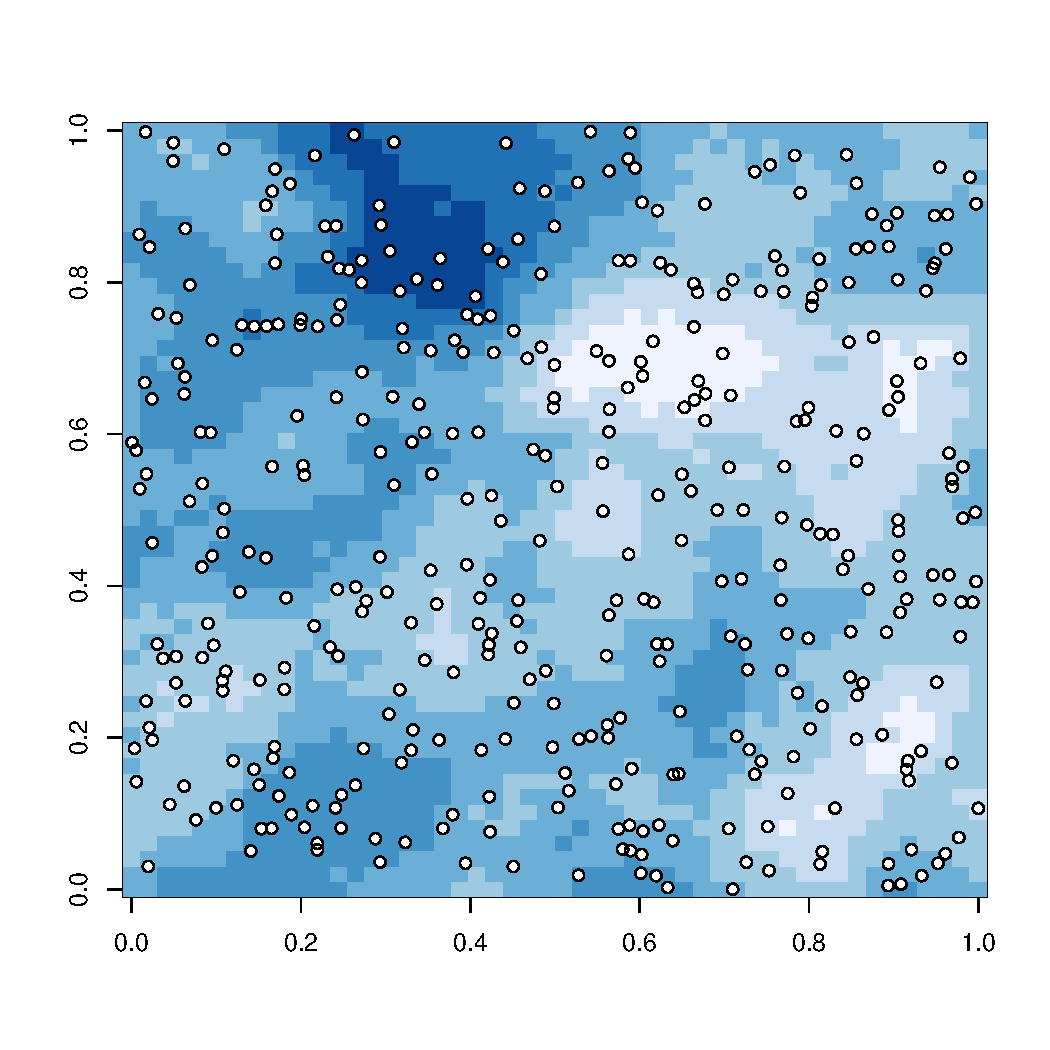
\includegraphics[width=0.95\textwidth]{locations.pdf}
  \caption{\small The locations $\bm{s}_1, \dots, \bm{s}_{400} \in \mathbb{R}^2$ of the observations from a Gaussian process with $\nu = 1.5$, $\rho = 0.1548$, and $\sigma = 1$. The locations are random, but generated in such a way that ensures the minimum distance between any two points is greater than $0.005$.}
  \label{fig:locations}
\end{figure}

\begin{figure}[!htb]
  \centering
  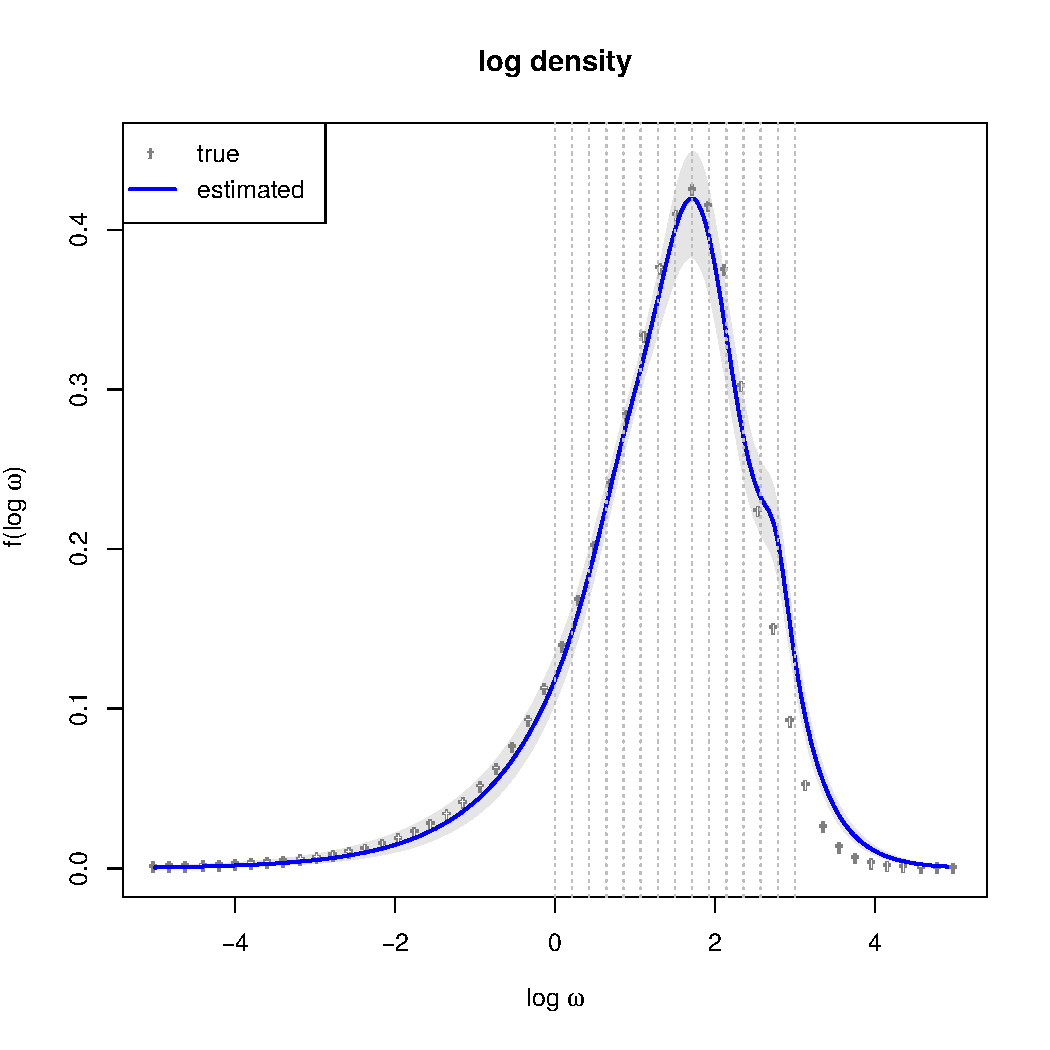
\includegraphics[width=0.95\textwidth]{logdensity2.pdf}
  \caption{\small The actual $f(\log \omega)$ (grey dots) versus the estimated $\hat{f}(\omega)$ (blue). The shaded area represents the range of the middle 95\% of $\hat{f}(\omega)$ for all draws from $\bm{\beta} \;|\; \bm{y}$. The vertical gray dotted lines indicate where the knots were placed.}
  \label{fig:result}
\end{figure}

\begin{figure}[!htb]
  \centering
  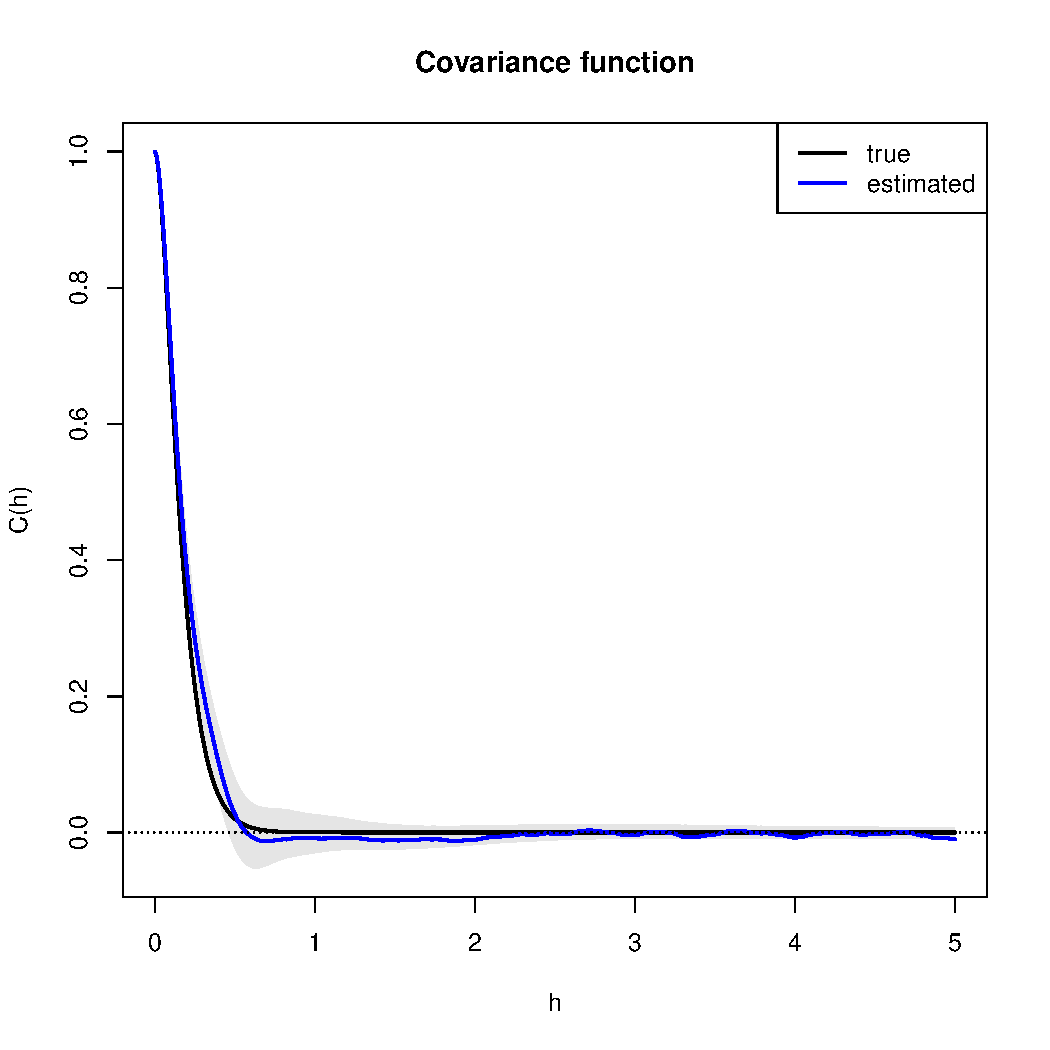
\includegraphics[width=0.95\textwidth]{covar.pdf}
  \caption{\small The actual $C(h)$ (black) versus the estimated $\widehat{C}(h)$ (blue). The shaded area represents the range of the middle 95\% of $\widehat{C}(h)$ for all draws from $\bm{\beta} \;|\; \bm{y}$.}
  \label{fig:result-covar}
\end{figure}

The overall simulation study was set up as follows: first we simulate 100 mean-zero Gaussian processes with Matern covariance functions ($\nu = 1.5, \rho = 0.1548, \sigma = 1$) and 100 mean-zero Gaussian processes with damped cosine covariance functions ($\lambda = 1, \tau = 1$) with 400 observations randomly placed over the unit square, as above. In addition, for every dataset, observations were generated over a $50\times50$ uniform grid. These were held out for prediction.

We compare three techniques. The first is the ``spline method'' from Section~\ref{section2:Procedure}. For the second, we fit a univariate Gaussian spatial regression model using the \texttt{spBayes} R package~\cite{spBayes1}~\cite{spBayes2}. This package's \texttt{spLM} function fits the model
\[
  y(\bm{s}) = \bm{x}(\bm{s})'\bm{\beta} + w(\bm{s}) + \varepsilon(\bm{s})
\]
using a Metropolis algorithm. See the package vignette for implementation details. In our case, we have no predictors $\bm{x}$, just the locations $\bm{s}$ themselves, so the model reduces to $y(\bm{s}) = w(\bm{s}) + \varepsilon(\bm{s})$, where $w$ is the spatial process and $\varepsilon$ is an independent white-noise process. We can specify that $w$ should employ a Mat\'{e}rn covariance function, and \texttt{spLM} can estimate the parameter values from \eqref{eq:matern}. In effect, this gives us the Mat\'{e}rn model that best fits the data.

The third technique is the one introduced by Hall et al.~\cite{Hall1994}. We find a kernel estimate of the covariogram using the kernel
\[
  K(x) = 0.9375(1 - x^2)^2
\]
as the authors do in their original paper. We then numerically calculate the Fourier transform of this covariagram estimate, set all values beyond the first nonnegative one to zero to ensure positive definiteness, and Fourier transform back to the spatial domain.

For each of these techniques, we estimate the covariance function using the 400 observations, generate predictions for the 2500 held out locations, and calculate the mean squared prediction error. We do this for every simulated dataset. Figure~\ref{fig:true-vs-est-all} shows the resulting covariance function estimates for every dataset, along with the true covariance functions. The Hall method underestimates the covariance at short distances in both the Mat\'{e}rn and damped cosine cases. Notice that the spline method is the only one to capture the hole effect in the damped cosine case, although it does tend to overestimate the magnitude of the effect.

\begin{figure}[htbp]
  \centering
  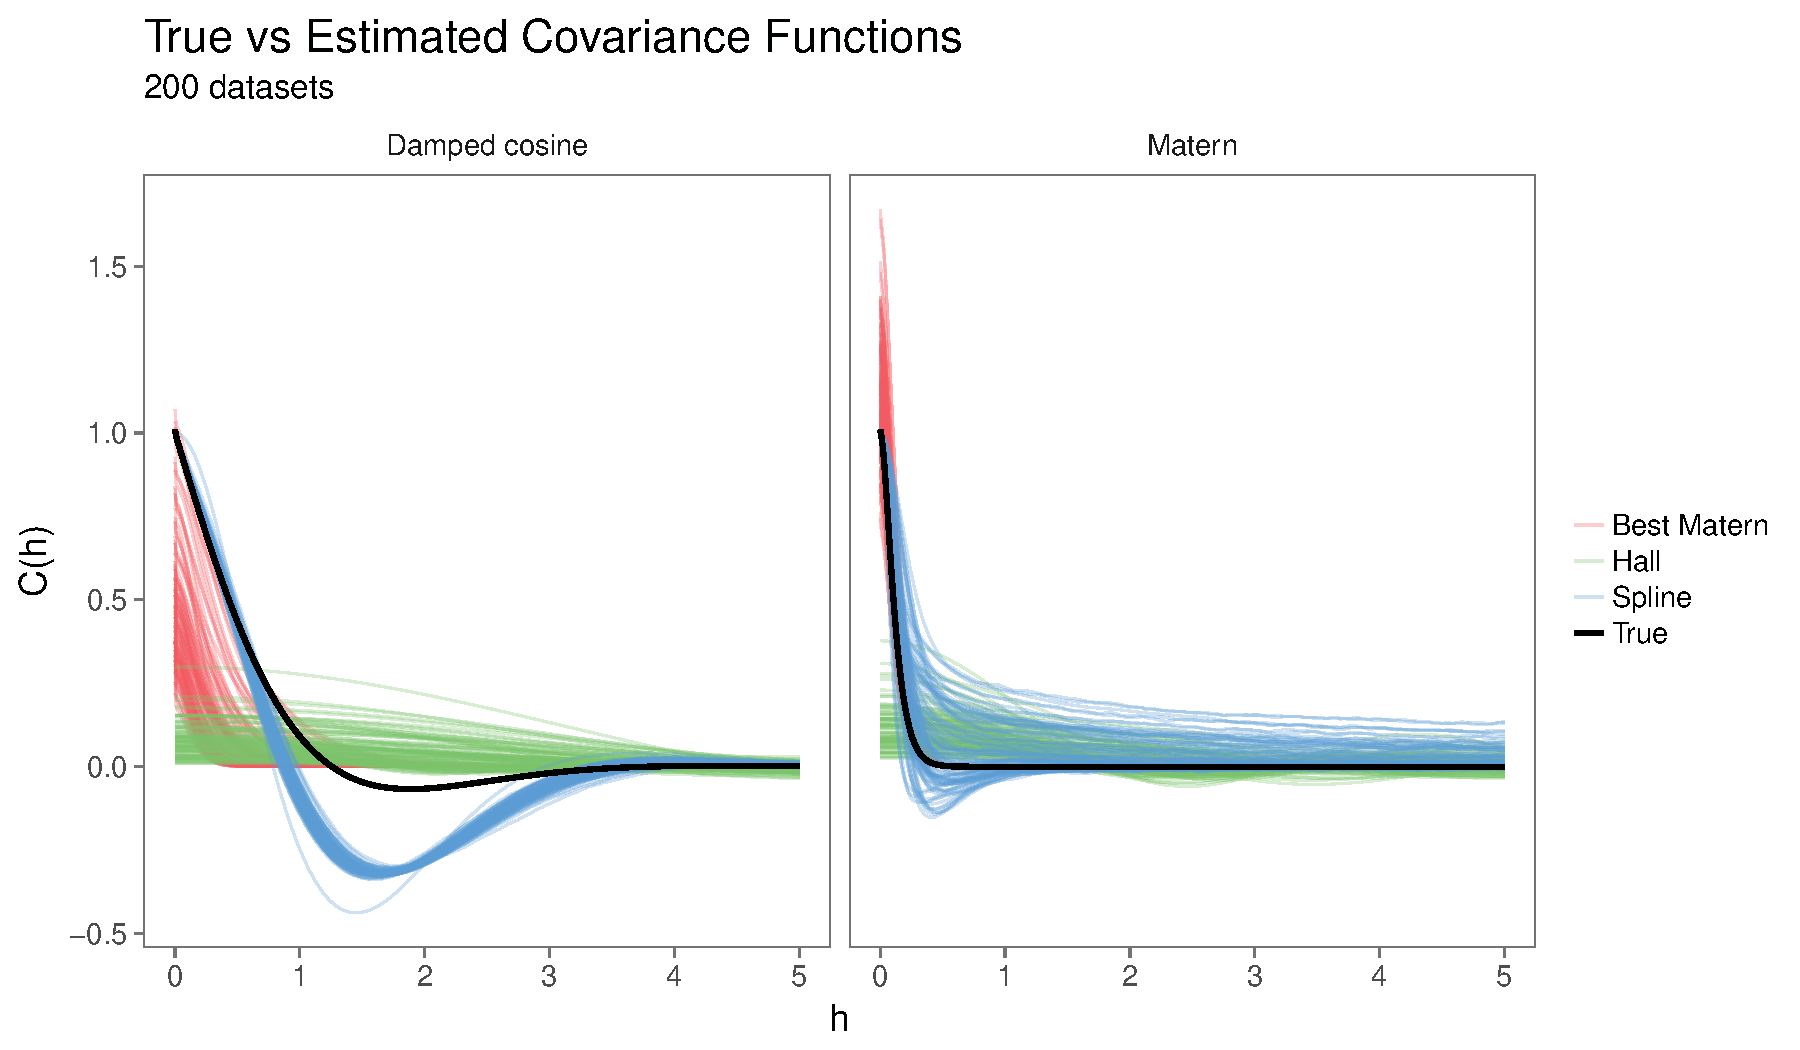
\includegraphics[width=0.95\textwidth]{true_vs_est_all.pdf}
  \caption{True covariance functions for the Mat\`{e}rn and damped cosine cases, along with all of the estimates. The spline method estimates are in blue, the Hall method is in green, and the best-fitting Mat\`{e}rn is in red.}
  \label{fig:true-vs-est-all}
\end{figure}

Finally, we examine the integrated mean-square prediction error (IMSPE). For each dataset, we calculate the \emph{optimal} IMSPE by generating predictions at each of the 2500 prediction locations according to the true covariance function, and then comparing them to the corresponding observations. The boxplots in Figure~\ref{fig:pred-log} show the IMSPE relative to this optimal value for every dataset. The IMSPE is shown on the log scale to make the boxplots a bit more readable relative to one another.

Notice that both the spline method and the best-fitting Mat\'{e}rn model outperform the Hall method with regard to prediction, and are fairly close to each other. As expected, the best-fitting Mat\'{e}rn performs the best when the true process was also Mat\'{e}rn. Interestingly, it performs a bit better than the spline method when the true process was not Mat\'{e}rn as well. This further validates the argument in~\cite{Stein1999} that the Mat\'{e}rn model is an excellent choice in most practical situations when prediction accuracy is the goal. It does not pick up the hole effect present at moderate distances in the damped cosine model (see Figure~\ref{fig:true-vs-est-all}), but interpolation is largely governed by the behavior at small distances, i.e. the smoothness of the process. The Mat\'{e}rn covariance function~\ref{eq:matern} has a parameter $\nu$ that controls this smoothness. Because we're estimating $\nu$ directly, we are able to precisely adjust it and get very good prediction performance.

There were a few Mat\'{e}rn datasets for which the spline method performed very poorly, as the long right tail of the boxplot indicates. This occurred when the Metropolis algorithm described in Algorithm~\ref{alg:mcmc} either mixed very poorly or started with poor initial $\bm{\beta}$ values. These issues could be corrected on any single dataset by manual intervention (e.g. by tuning the algorithm, running more iterations, etc.), but because the method was applied to all 100 datasets in bulk, we did not tune them individually. Note that these issues arose in only a few datasets, and the median relative IMSPE is still competitive with the best-fitting Mat\'{e}rn results.

\begin{figure}[htbp]
  \centering
  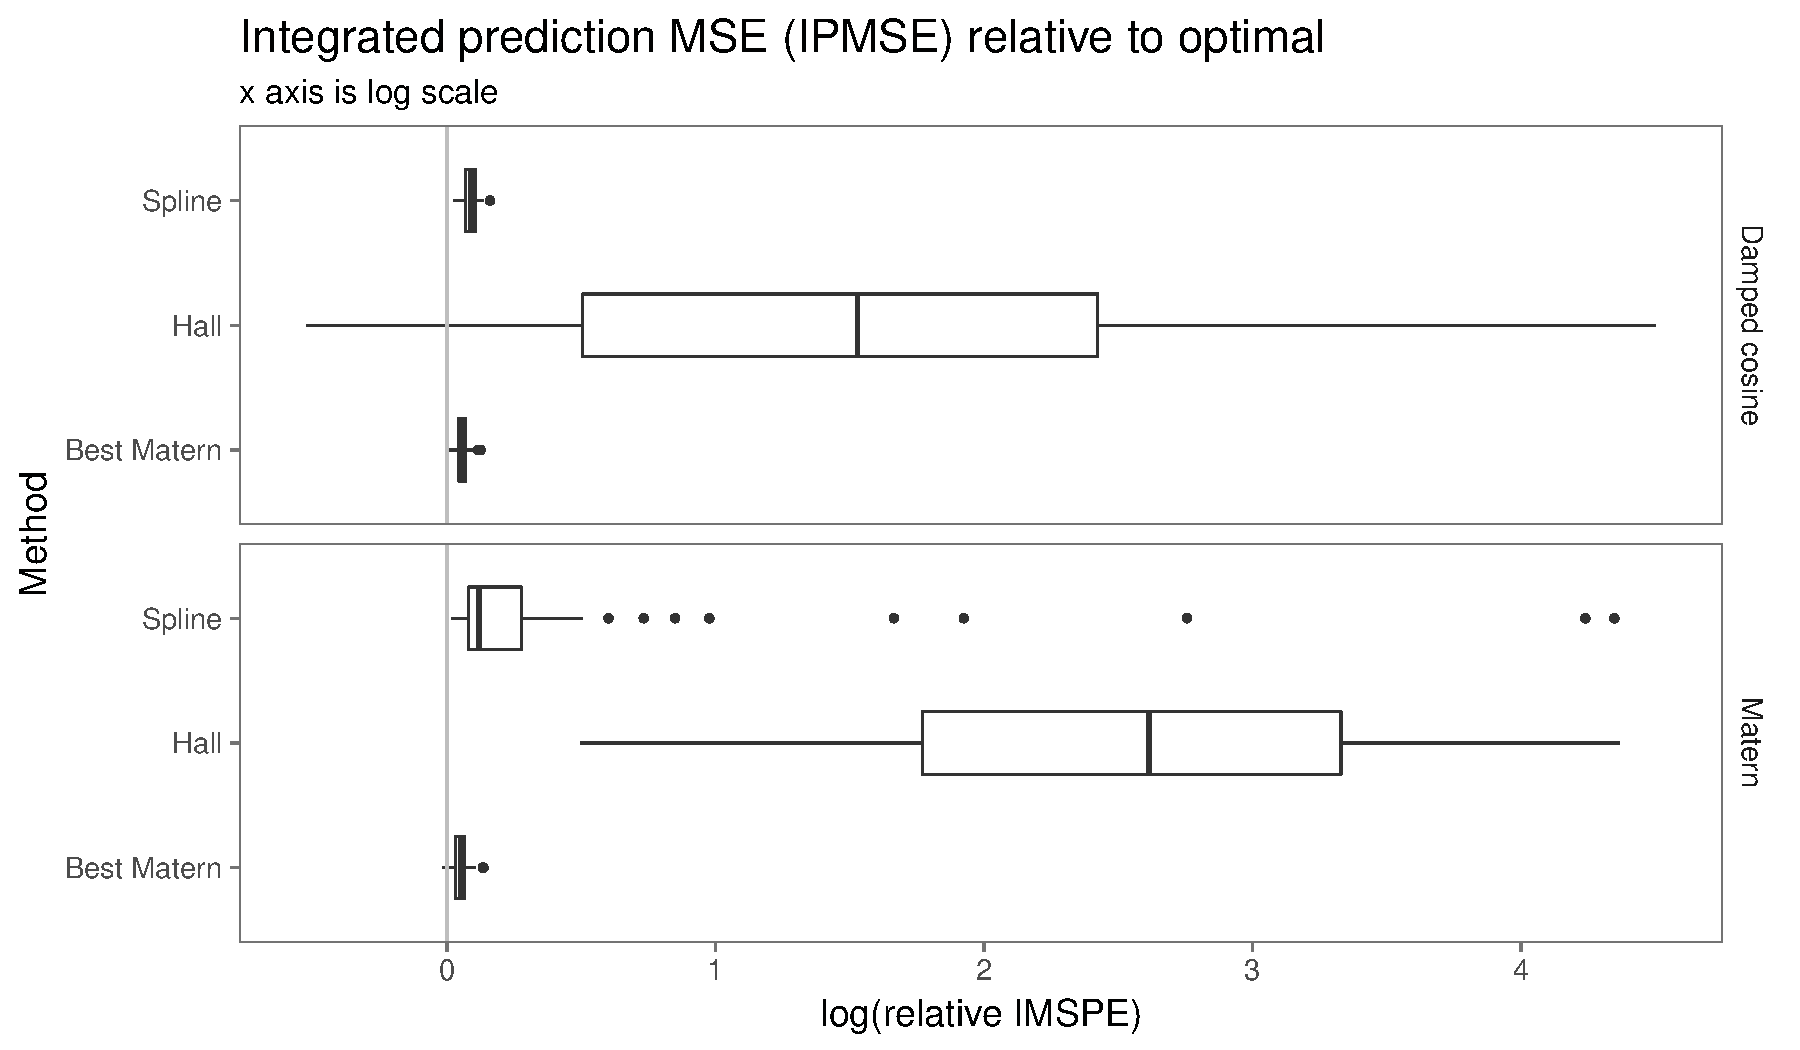
\includegraphics[width=0.95\textwidth]{pred_log.pdf}
  \caption{Mean squared prediction error relative to the optimal. The x axis is on the log scale, so the optimal MSPE would fall at zero.}
  \label{fig:pred-log}
\end{figure}

\subsection{Covariance Function Estimation Performance} % (fold)
\label{sec:covariance_function_estimation_performance}

We continue to evaluate these techniques by introducing another measure of performance. Broadly, we would like to know how closely the estimated covariance function aligns with the true covariance function. Let $C(h)$ be the true covariance and $\widehat{C}_m(h)$ be the estimate from method $m$. Define the function
\[
  g_m(h) = \big(C(h) - \widehat{C}_m(h) \big)^2.
\]
Then the integrated mean squared error with respect to method $m$ is
\[
  IMSE_m = \int_0^\infty g_m(h) \; dh.
\]
To approximate this integral, we evaluate $g_m(h)$ on a uniform grid $\{h_0, \dots, h_N\}$, $0 \leq h_i \leq 5$, and use the trapezoidal rule:
\[
  \widehat{IMSE}_m = \sum_{i=1}^N \frac{g_m(h_{i-1}) + g_m(h_i)}{2} (h_i - h_{i-1}).
\]
In Figure~\ref{fig:sqdiff}, the functions $g_m(h)$ are shown for all methods and both covariance function types.

\begin{figure}[htbp]
  \centering
  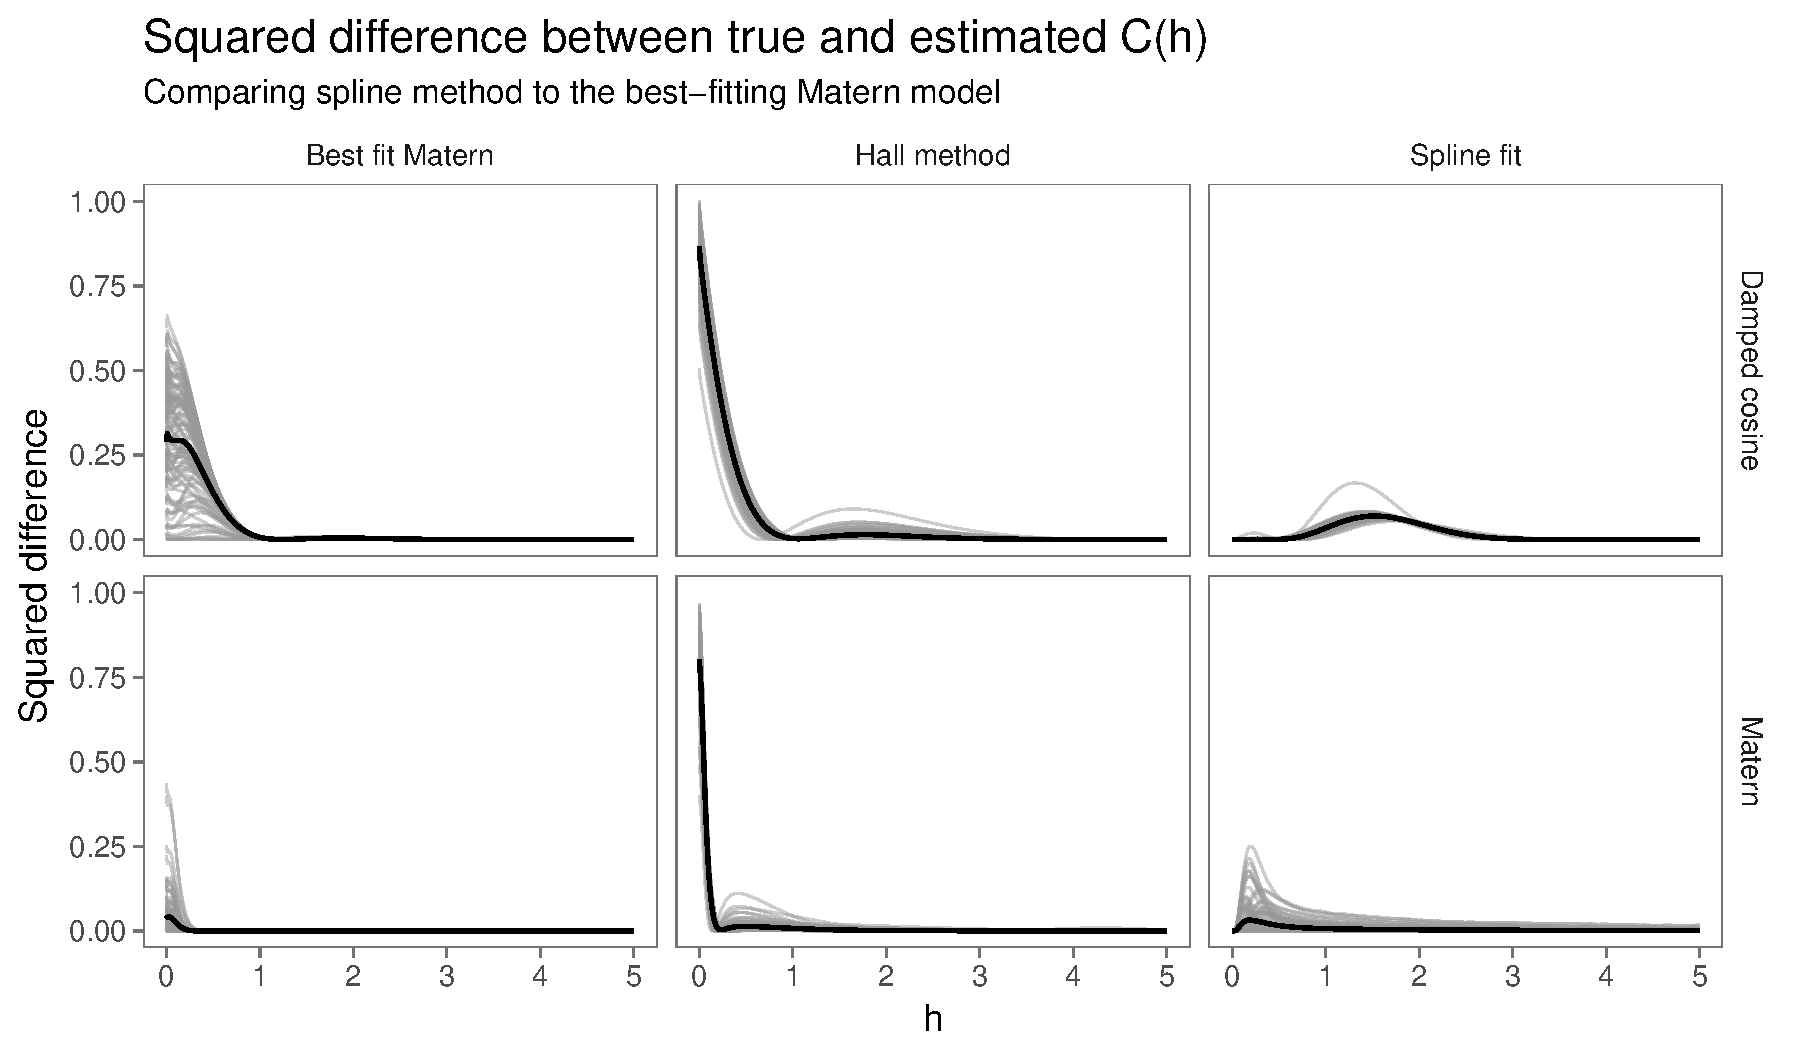
\includegraphics[width=0.95\textwidth]{sqdiff.pdf}
  \caption{Squared discrepancy functions $g_m(h)$ for every method, both Mat\'{e}rn and damped cosine covariance models. The result from each simulated dataset is shown in gray, and the thicker black lines are the means of each facet of the plot.}
  \label{fig:sqdiff}
\end{figure}

There are a number of interesting features of this figure. First of all, the squared difference functions of the best-fit Mat\'{e}rn model and the spline method are, for the most part, quite small in magnitude. This further confirms what we observed in Figure~\ref{fig:true-vs-est-all} that these two methods fit the true Mat\'{e}rn covariance function very well. The Hall method does not perform as well for small $h$, although it does recover and match the true function once $h$ is greater than 2. The best-fit Mat\'{e}rn tends to be slightly inaccurate for very small $h$, but its errors are smaller and it recovers even more quickly than the Hall method. On the other hand, the spline method appears to be at its most inaccurate not at $h = 0$, but around $0.25 < h < 1$.

Not surprisingly, the best-fit Mat\'{e}rn does not match the true covariance as well when the truth is not actually a Mat\'{e}rn covariance function. The spline method is closer to the truth, but it does tend to consistently overestimate the magnitude of the hole effect at $1 < h < 2$. The Hall method is the least accurate of the three on these data.

Figure~\ref{fig:boxplot-integrals} shows the IMSE (the integrals of the curves in Figure~\ref{fig:true-vs-est-all}) for all datasets. Again, the best-fit Mat\'{e}rn and the spline method performed comparably on the Mat\'{e}rn datasets, with the Hall method doing worse. For the damped cosine datasets, the spline method performed better on average than the best-fit Mat\'{e}rn.

\begin{figure}[htbp]
  \centering
  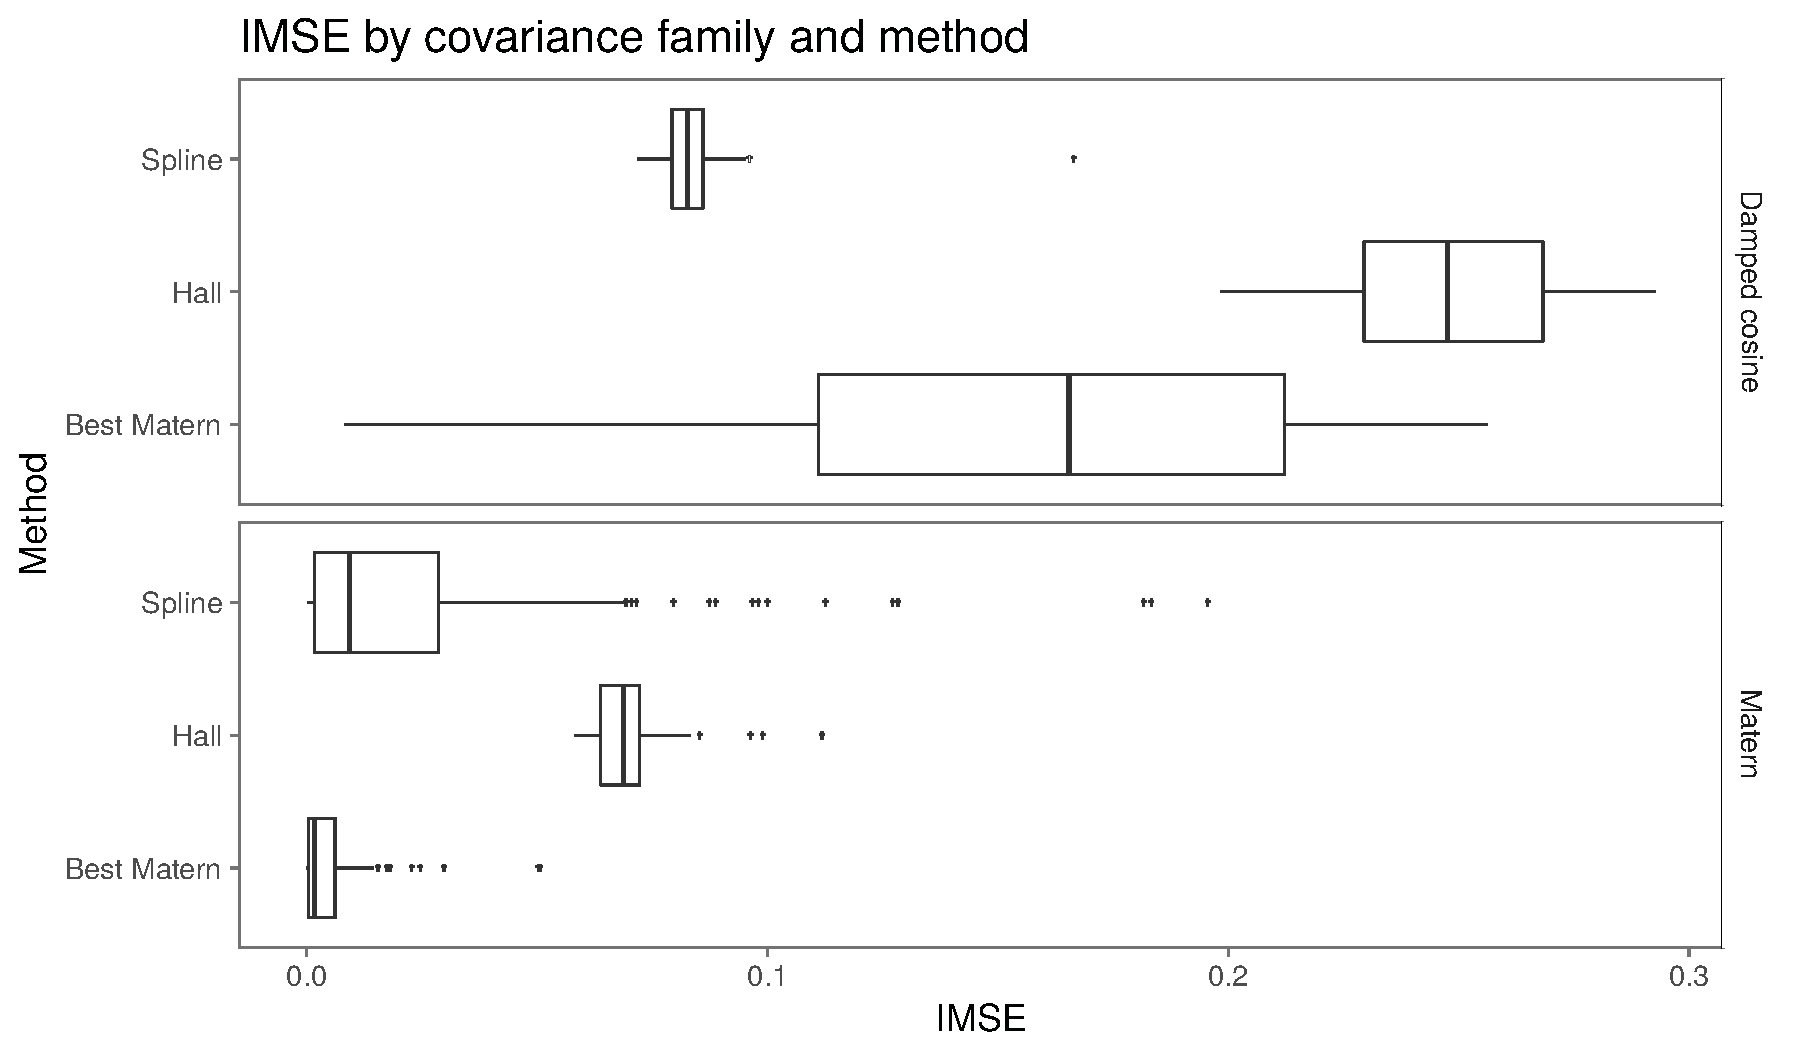
\includegraphics[width=0.95\textwidth]{boxplot_integrals2.pdf}
  \caption{Boxplots of IMSE by method.}
  \label{fig:boxplot-integrals}
\end{figure}

% section covariance_function_estimation_performance (end)

\section{Data Application}
\label{section4:Data-Application}

To evaluate the performance of our method on real data, we use an atomic force microscopy (AFM) image of a solar cell. The image (see Figure~\ref{fig:film}) comes from a paper by Singh et al.~\cite{Singh2014}, who wanted to improve efficiency of converting light into electricity by optimizing the concentration of carbon nanotubes in solar cells coated with a particular compound called poly(3-hexylthiophene): phenyl-C61-butyric acid methyl ester (P3HT:PCBM). This compound is spread in a microscopically thin film over the cell.

\begin{figure}[htbp]
  \centering
  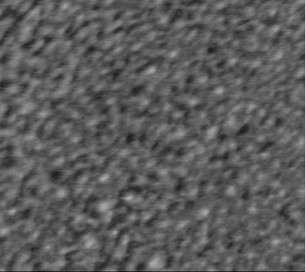
\includegraphics[width=0.65\textwidth]{film.png}
  \caption{Atomic force microscopy image of a thin film of the P3HT:PCBM compound on a solar cell. Dark clusters represent areas where the film is thinner, and lighter clusters are thicker areas.}
  \label{fig:film}
\end{figure}

Figure~\ref{fig:film} shows a P3HT:PCBM film doped with a 0.1\% concentration of carbon nanotubes. By treating the film thickness as observations from an unknown isotropic stationary Gaussian process, our goal was to train a covariance model on some of these observations and predict the others.

To prepare the data, we selected ten 25-by-25 pixel squares to use to estimate the covariance function. We treated the squares as 10 independent observations of a Gaussian process on the 25-by-25 grid. Once we obtained our estimate, we selected an out of sample 25-by-25 square, removed a 4-by-4 section of that square made predictions conditionally on the remainder as observations in the square. One of the training squares is shown in Figure~\ref{fig:training25}, and Figure~\ref{fig:pred25} shows the observation square, with the withheld prediction points highlighted in red.

\begin{figure}[htbp]
  \centering
  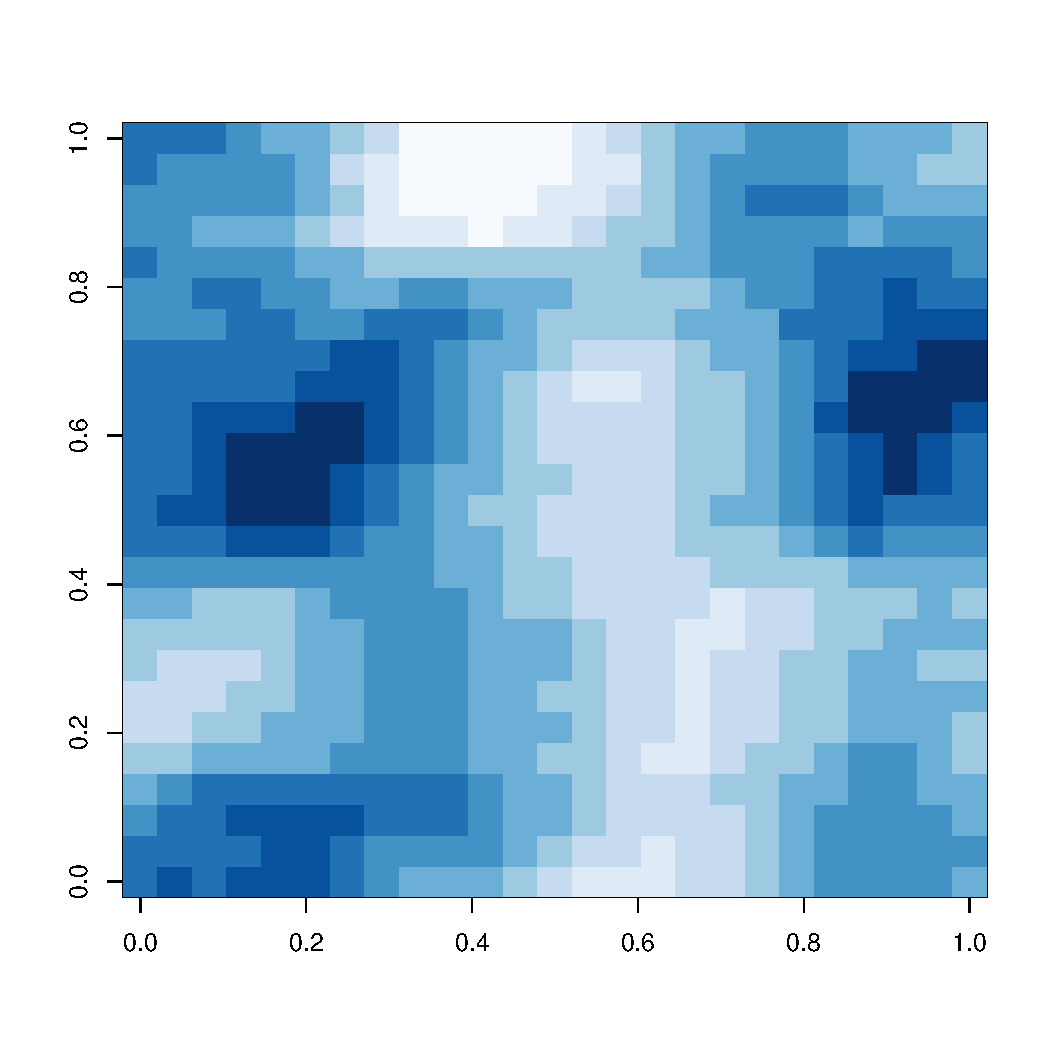
\includegraphics[width=0.95\textwidth]{col_image_5.pdf}
  \caption{One of the 10 25-by-25 sections of the film image used to fit the spline model.}
  \label{fig:training25}
\end{figure}

\begin{figure}[htbp]
  \centering
  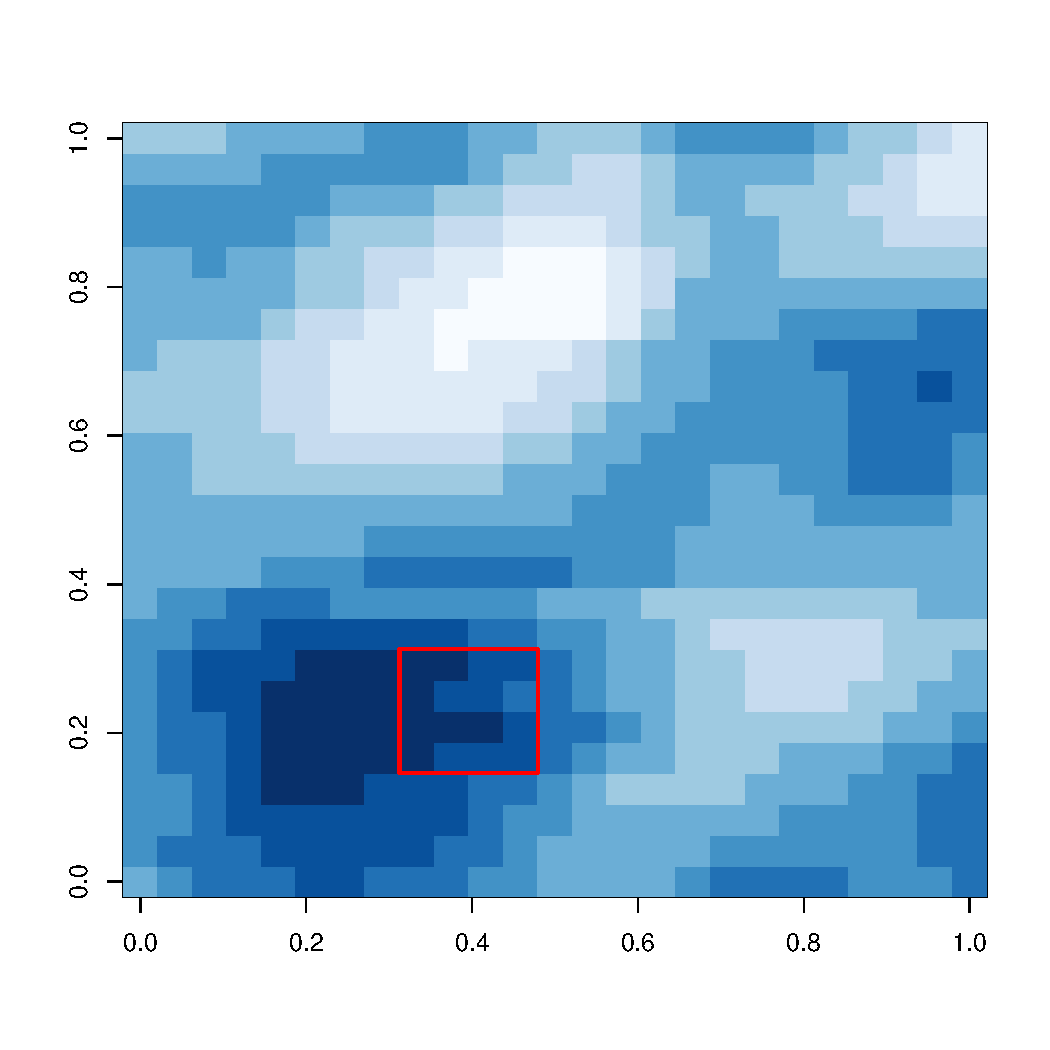
\includegraphics[width=0.95\textwidth]{col_pred.pdf}
  \caption{This 25-by-25 section of the film image was held out from the training step. The 16 outlined pixels are used for prediction, and the others are treated as observations.}
  \label{fig:pred25}
\end{figure}

\begin{figure}[htbp]
  \centering
  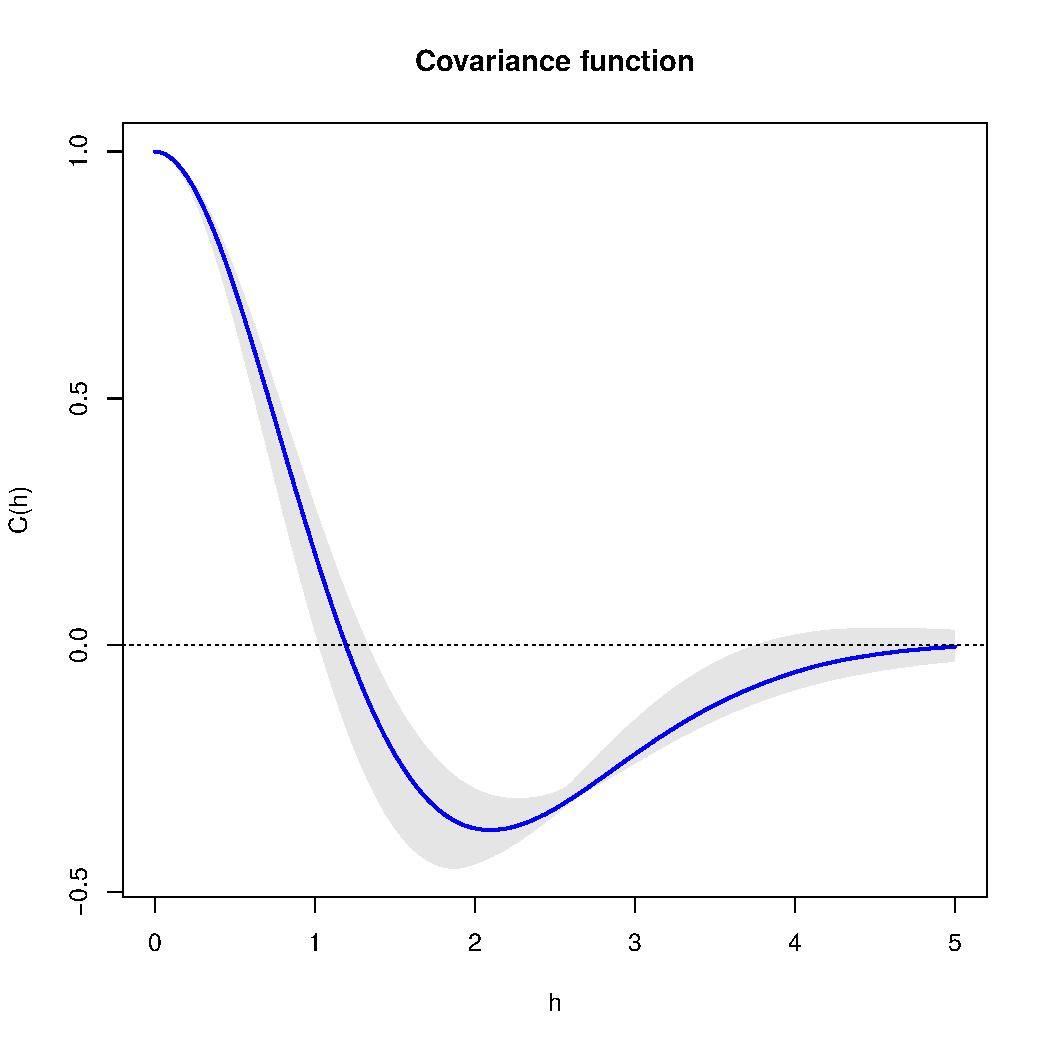
\includegraphics[width=0.95\textwidth]{covariance_realdata.pdf}
  \caption{The estimated covariance function based on the 10 25-by-25 sections of the film image used to fit the spline model.}
  \label{fig:covariance-realdata}
\end{figure}

We fit the semiparametric model and a Mat\'ern model, and compare the prediction performance of each. The mean squared prediction error for the Mat\'ern model was $0.0008707$, while the mean squared prediction error for the semiparametric model was $0.0006414$. The semiparametric model performed $26.3\%$ better on the 16 prediction points, indicating that it is capturing the local behavior of the Gaussian process more effectively than the best-fit Mat\'ern model can. Figure~\ref{fig:covariance-realdata} shows the estimated covariance function from the semiparametric model. There is a significant hole effect that a Mat\'ern model is not capable of capturing.


\section{Conclusions and Future Work}
\label{section5:Conclusions}

This paper presents a method for estimating the covariance function of a stationary isotropic Gaussian process that does not rely on choosing a parametric family that may or may not fit the data well. It allows the data alone to drive the estimation, yet still guarantees that the estimated covariance function will turn out to be positive definite.

It is generally believed~\cite{Stein1999} that fitting a Mat\'ern covariance function, via maximum likelihood or something similar, will give good interpolation performance even if the covariance of the true underlying Gaussian process can't be approximated very closely by a function from the Mat\'ern family. Our simulations in Section~\ref{section3:Simulation-Study} support that claim. However, our method has performed comparably with regard to prediction (Figure~\ref{fig:pred-log}). In addition, we observed that our method can more closely match the covariance function (Figure~\ref{fig:boxplot-integrals}) in cases where a "hole effect", or distances that correspond to a negative covariance, exists. One example of this phenomenon is the damped cosine covariance function \eqref{eq:dampedcos}.

Our method involves estimating the covariance matrix element by element, which is an extremely computationally intensive problem, and one that would scale quite poorly if it were executed sequentially. However, this issue is largely alleviated through the use of parallel computing on a GPU. For a moderately sized problem (here $n = 400$), the GPU approach results in a speedup of roughly $100\times$. %Also, we expect that as the number of observations increases, our method would outperform other methods in terms of speed

% \section{Future Work} % (fold)
% \label{sec:future_work}

This semiparametric covariance estimation method could be adapted to allow us to relax the isotropy and stationarity assumptions. Modeling an anisotropic Gaussian process would be a straightforward extension; it would involve replacing the simplification in \eqref{eq:bochner2} with a two-dimensional Fourier transform
\[
  C(\bm{h}) = \iint_{-\infty}^{\infty} \exp(i\bm{h}^T\bm{\omega}) \; f(\bm{\omega}) \; d\bm{\omega}.
\]

It is possible to relax the stationarity assumption as well. In the literature there are several methods for dealing with spectral densities of nonstationary Gaussian processes. One notable example is the work of Fuentes~\cite{fuentes2002spectral}, who proposed a nonstationary periodogram that is a nonparametric estimator of the spectral density $f(\omega_1, \omega_2)$.

% This project is still a work in progress. As mentioned in Section~\ref{sec:calculating_the_likelihood}, I am working on a formal proof that the estimated likelihood converges to the true likelihood. In addition, I believe the performance of Algorithm~\ref{alg:mcmc} could be improved. The results in Figure~\ref{fig:result} are disappointing, but I think it could be more accurate with better proposal distributions and/or better knot placement. It could use more tinkering.

% The overall speed could be improved as well. Currently the MCMC algorithm runs in R, and invokes a CUDA C function to perform the Monte Carlo integrations. Translating all of the code into C/C++ would improve the performance even further. In particular, there is a matrix inversion via Cholesky decomposition in the likelihood calculation. It's possible to implement that in parallel on a GPU as well, which would allow $n$ to be larger than $400$ without harming performance too much.

% Finally, we would like to be able to relax the assumptions on the Gaussian process. We still need stationarity, but it should be a straighforward extension to eliminate the need to assume the process is isotropic.

% subsection future_work (end)

\bigskip
\begin{center}
{\large\bf SUPPLEMENTAL MATERIALS}
\end{center}

\begin{lemma} \label{lem:meanconcave}
  Let $f$ be a real-valued function that is continuous on $[a, b]$, differentiable on $(a, b)$, and concave over $(a, b)$. Then
  \[
    f(x) - f(\xi) \leq f'(\xi) (x - \xi) \qquad \forall \xi \in (a, b).
  \]
\end{lemma}

\begin{proof}
  \textsc{Case 1.} Suppose $x > \xi$. By the mean value theorem, there exists some $\eta \in (\xi, x)$ such that
  \[
    f'(\eta) = \frac{f(x) - f(\xi)}{x - \xi}.
  \]
  Since $f$ is concave, $f'$ is a decreasing function. Therefore $f'(\eta) \leq f'(\xi)$, and so
  \[
    f(x) - f(\xi) \leq f'(\xi) (x - \xi).
  \]
  \textsc{Case 2.} Suppose $x < \xi$. By the mean value theorem, there exists some $\eta \in (x, \xi)$ such that
  \[
    f'(\eta) = \frac{f(\xi) - f(x)}{\xi - x}.
  \]
  Since $f$ is concave, $f'$ is a decreasing function. Therefore $f'(\eta) \geq f'(\xi)$, and so
  \begin{align*}
    f(\xi) - f(x) &\geq f'(\xi) (\xi - x) \\
    f(x) - f(\xi) &\leq f'(\xi) (x - \xi).
  \end{align*}
\end{proof}

\begin{lemma} \label{lem:logineq}
  For all $x \in (0, \infty)$,
  \[
    \log x \leq x - 1.
  \]
\end{lemma}

\begin{proof}
  $f(x) = \log x$ is a concave function over the interval $(0, \infty)$. Use Lemma~\ref{lem:meanconcave} with $\xi = 1$.
  \begin{align*}
    \log x - \log 1 &\leq \frac{d}{dx}(\log x) \Big|_{x=1} (x - 1) \\
    \log x - 0 &\leq 1 (x - 1) \\
    \log x &\leq x - 1.
  \end{align*}
\end{proof}

Let $\bm{Y} = (Y_1, \dots, Y_n)^T$ be a random vector consisting of observations from a stationary, isotropic Gaussian process with mean 0 and covariance function $C$. The observations are located at $\bm{s}_1, \dots, \bm{s}_n \in \mathcal{D} \subseteq \mathbb{R}^d$ in some bounded domain $\mathcal{D}$. Then the distribution of $\bm{Y}$ is
\[
  \bm{Y} \sim \mathcal{N}_n(0, \bm{\Sigma})
\]
where $\Sigma_{ij} = C(||\bm{s}_i - \bm{s}_j||) = C(h_{ij})$. The likelihood function is
\[
  \ell(\bm{\Sigma}; \bm{y}) = -\frac{n}{2} \log(2\pi) - \frac{1}{2} \log \textrm{det}(\bm{\Sigma}) - \frac{1}{2} \bm{y}^T \bm{\Sigma}^{-1} \bm{y}.
\]




\begin{theorem}
  Let $\bm{y} = (y_1, \dots, y_n)^T$ be a vector of observations from a mean-zero stationary, isotropic Gaussian process with covariance function $C(h)$, taken at locations $\bm{s}_1, \dots, \bm{s}_n \in \mathcal{D} \subseteq \mathbb{R}^d$ in some bounded domain $\mathcal{D}$.  For some symmetric density $f(\omega)$, let $\ell(\bm{y})$ be the likelihood
  \[
    \ell(\bm{y}) = -\frac{n}{2} \log(2\pi) - \frac{1}{2} \log(|\bm{\Sigma}|) - \frac{1}{2} \bm{y}^T \bm{\Sigma}^{-1} \bm{y},
  \]
where $\Sigma_{ij} = \int \cos(h_{ij}\omega)f(\omega)d\omega$, and $\hat{\ell}(\bm{y})$ be the Monte Carlo approximated likelihood
    \[
    \hat{\ell}(\bm{y}) = -\frac{n}{2} \log(2\pi) - \frac{1}{2} \log (| \widehat{\bm{\Sigma}}|) - \frac{1}{2} \bm{y}^T \widehat{\bm{\Sigma}}^{-1} \bm{y}
  \] 
where $\widehat{\Sigma}_{ij} = \frac{1}{M} \sum_{m=1}^M \cos(\widetilde{\omega}_m h_{ij})$, and $\widehat{\omega}_1, \dots, \widehat{\omega}_M$ are an iid sample from $f(\omega)$.  Then as $M \to \infty$,
\[
\hat{\ell}(\bm{y}) \to \ell(\bm{y}) \text{ a.s. }f_\omega.
\]
\end{theorem}

\begin{proof}

We will show that
\[
\Big|\hat{\ell}(\bm{\beta}; \bm{y}) - \ell(\bm{\Sigma}; \bm{y})\Big| = -\frac{1}{2} \Big| \log \textrm{det}(\widehat{\bm{\Sigma}}) - \log \textrm{det}(\bm{\Sigma}) \Big| - \frac{1}{2} \bm{y}^T \Big| \widehat{\bm{\Sigma}}^{-1} - \bm{\Sigma}^{-1} \Big| \bm{y} \to 0.
\]
The notation in the final term refers to
\[
  \Big| \widehat{\bm{\Sigma}}^{-1} - \bm{\Sigma}^{-1} \Big| =
  \begin{bmatrix}[2]
    \Big| \widehat{\Sigma}^{-1}_{11} - \Sigma^{-1}_{11} \Big| & \Big| \widehat{\Sigma}^{-1}_{12} - \Sigma^{-1}_{12} \Big| & \cdots \\
    \Big| \widehat{\Sigma}^{-1}_{21} - \Sigma^{-1}_{21} \Big| & \Big| \widehat{\Sigma}^{-1}_{22} - \Sigma^{-1}_{22} \Big| & \cdots \\
    \vdots & \vdots & \ddots
  \end{bmatrix}.
\] \label{symb:absmat}
Consider the first term. Let $\lambda_1, \dots, \lambda_n$ and $\hat{\lambda}_1, \dots, \hat{\lambda}_n$ be the eigenvalues of $\bm{\Sigma}$ and $\widehat{\bm{\Sigma}}$ respectively.
\[
  \Big| \log \textrm{det}(\widehat{\bm{\Sigma}}) - \log \textrm{det}(\bm{\Sigma}) \Big| = \left| \sum_{i=1}^n \log \hat{\lambda}_i - \sum_{i=1}^n \log \lambda_i \right| = \left| \sum_{i=1}^n \log \frac{\hat{\lambda}_i}{\lambda_i} \right|.
\]
From Lemma~\ref{lem:logineq},
\begin{align*}
  \sum_{i=1}^n \log \frac{\hat{\lambda}_i}{\lambda_i} &\leq \sum_{i=1}^n \left( \frac{\hat{\lambda}_i}{\lambda_i} - 1 \right) \\
  &= \sum_{i=1}^n \frac{\hat{\lambda}_i - \lambda_i}{\lambda_i} \\
  &\leq \sum_{i=1}^n \frac{|\hat{\lambda}_i - \lambda_i|}{\lambda_i} \\
  &\leq \sqrt{\sum_{i=1}^n (\hat{\lambda}_i - \lambda_i)^2} \sqrt{\sum_{i=1}^n \frac{1}{\lambda_i^2}}. \tag{Cauchy-Schwarz}
\end{align*}
Because for all $i,j$, $\widehat{\Sigma}_{ij} \xrightarrow[M \to \infty]{} \Sigma_{ij}$ uniformly a.s. $f_\omega$, the Frobenius norm 
\[
  ||\widehat{\bm{\Sigma}} - \bm{\Sigma}||_F = \sqrt{\sum_{i=1}^n \sum_{j=1}^n \left| \widehat{\Sigma}_{ij} - \Sigma_{ij} \right|^2} \xrightarrow[M \to \infty]{} 0.
\]
Theorem 4.2.8 of~\cite{hsing2015theoretical} tells us that
\[
  \sup_{k \geq 0} |\hat{\lambda}_{k+1} - \lambda_{k+1}| \leq ||\widehat{\bm{\Sigma}} - \bm{\Sigma}||.
\]
Therefore
\begin{align*}
  \sup_{k \geq 0} |\hat{\lambda}_{k+1} - \lambda_{k+1}| &\to 0 \\
  \sum_{i=1}^n (\hat{\lambda}_i - \lambda_i)^2 &\to 0 \\
  \Big| \log \textrm{det}(\widehat{\bm{\Sigma}}) - \log \textrm{det}(\bm{\Sigma}) \Big| &\to 0 \quad \textrm{a.s. } f_\omega.
\end{align*}

Now consider the second term. We need to show that
\[
  \bm{y}^T \Big| \widehat{\bm{\Sigma}}^{-1} - \bm{\Sigma}^{-1} \Big| \bm{y} \xrightarrow[M \to \infty]{} 0.
\]
\begin{align*}
  \Big|\Big| \bm{y}^T \big| \widehat{\bm{\Sigma}}^{-1} - \bm{\Sigma}^{-1} \big| \bm{y} \Big|\Big| &\leq ||\widehat{\bm{\Sigma}}^{-1} - \bm{\Sigma}^{-1}|| \; ||\bm{y}||^2 \\
  &\leq || \widehat{\bm{\Sigma}}^{-1} \bm{\Sigma} \bm{\Sigma}^{-1} - \widehat{\bm{\Sigma}}^{-1} \widehat{\bm{\Sigma}} \bm{\Sigma}^{-1} || \; ||\bm{y}||^2 \\
  &\leq || \widehat{\bm{\Sigma}}^{-1} (\bm{\Sigma} - \widehat{\bm{\Sigma}}) \bm{\Sigma}^{-1} || \; ||\bm{y}||^2 \\
  &\leq || \widehat{\bm{\Sigma}}^{-1} || \; || \bm{\Sigma} - \widehat{\bm{\Sigma}} || \; || \bm{\Sigma}^{-1} || \; ||\bm{y}||^2.
\end{align*}
As previously shown, $|| \bm{\Sigma} - \widehat{\bm{\Sigma}} || \xrightarrow[M \to \infty]{} 0$, so
\[
  \bm{y}^T \Big| \widehat{\bm{\Sigma}}^{-1} - \bm{\Sigma}^{-1} \Big| \bm{y} \xrightarrow[M \to \infty]{} 0 \quad \textrm{a.s. } f_\omega
\]
as desired.

\end{proof}

\begin{description}

\item[Title:] Brief description. (file type)

\item[R-package for  MYNEW routine:] R-package ÒMYNEWÓ containing code to perform the diagnostic methods described in the article. The package also contains all datasets used as examples in the article. (GNU zipped tar file)

\item[HIV data set:] Data set used in the illustration of MYNEW method in Section~ 3.2. (.txt file)

\end{description}

% \begin{thebibliography}{}

% \bibitem[Azzalini(2005)]{azza:05}
% Azzalini, A. (2005).
% \newblock The skew-normal distribution and related multivariate families.
% \newblock \emph{Scandinavian Journal of Statistics} \textbf{32}, 159--188.

% \end{thebibliography}{}

\bibliography{report}

\end{document} 